\documentclass[notes,blackandwhite,mathsans,usenames,dvipsnames]{beamer}

\usepackage{amsmath}
\usepackage{amssymb}
\usepackage{graphicx}
\usepackage{fancybox}
\usepackage{booktabs}
\usepackage{multirow,pxfonts}
\usepackage{cmbright}
\usepackage{xcolor}
\usepackage{color}
\usepackage{enumitem}
\usepackage{animate}
\usepackage{changepage}
\usepackage{wrapfig}
\usepackage{array}


\usepackage[T1]{fontenc}
\fontencoding{T1}  
\usepackage[utf8]{inputenc}


\usefonttheme{default}
\setbeamercovered{invisible}
\beamertemplatenavigationsymbolsempty

\makeatletter
\setbeamertemplate{footline}
{
  \leavevmode
  \hbox{
  \begin{beamercolorbox}[wd=0.97\paperwidth,ht=2.25ex,dp=2ex,right]{}
{\color{mcxs2} \insertframenumber{} / \inserttotalframenumber}
  \end{beamercolorbox}}%
}


\definecolor{mcxs1}{HTML}{05386B}
\definecolor{mcxs2}{HTML}{379683}
\definecolor{mcxs3}{HTML}{5CDB95}
\definecolor{mcxs4}{HTML}{8EE4AF}
\definecolor{mcxs5}{HTML}{EDF5E1}
\setbeamercolor{frametitle}{fg=mcxs2}
\AtBeginDocument{\color{mcxs1}}
\setbeamertemplate{itemize item}[triangle]



\begin{document}
%\fontfamily{pag}\selectfont
%\setbeamerfont{title}{family=\fontfamily{pag}\selectfont}
%\setbeamerfont{frametitle}{family=\fontfamily{pag}\selectfont}
%\setbeamerfont{framesubtitle}{family=\fontfamily{pag}\selectfont}






{\setbeamercolor{background canvas}{bg=mcxs1}
\begin{frame}

\vspace{1cm}
\begin{tabular}{rl}
&\textbf{\LARGE\color{mcxs2} Macroeconometrics}\\[8ex]
\textbf{\Large\color{purple} Lecture 15}&\textbf{\Large\color{mcxs2}Modeling effects of monetary policy}\\[16ex]
&\textbf{\color{purple}Tomasz Wo\'zniak}\\[1ex]
&{\small\color{mcxs3} Department of Economics}\\
&{\small\color{mcxs3}University of Melbourne}
\end{tabular}

\end{frame}
}




{\setbeamercolor{background canvas}{bg=mcxs1}
\begin{frame}

\vspace{1cm}\textbf{\color{mcxs2}A small-open economy model revisited}

\bigskip\textbf{\color{purple}Modeling effects of monetary policy in the US}

\bigskip\textbf{\color{mcxs2}Modeling effects of monetary policy in the US\\ $\qquad$-- extended analysis}


%\small
%\vspace{1cm} Compulsory readings: \scriptsize
%
%\smallskip{\color{mcxs2}Wo\'zniak (2019) Bayesian Structural VARs: Algorithms and Inference, Lecture notes}


%\bigskip Useful readings: \scriptsize
%
%\smallskip{\color{mcxs2}Waggoner \& Zha (2003) A Gibbs sampler for structural vector autoregressions, Journal of Economic Dynamics \& Control}

%\smallskip{\color{mcxs2}Waggoner \& Zha (2003) Likelihood preserving normalization in multiple equation models, Journal of Econometrics}

%\normalsize
\vspace{2cm}{\color{mcxs2}Materials: }

\smallskip{\color{mcxs2}A zip file} \texttt{\color{purple}L15 mcxs-all.zip} {\color{mcxs2}for the reproduction of the results}

\end{frame}
}



{\setbeamercolor{background canvas}{bg=mcxs2}
\begin{frame}

\bigskip\textbf{\color{mcxs1}Objectives.}
\begin{itemize}[label=$\blacktriangleright$]
\item {\color{mcxs1}To present the outcomes of Waggoner \& Zha (2003) estimation algorithm}
\item {\color{mcxs1}To work with a variation on the small-open economy model}
\item {\color{mcxs1}To investigate the effects of the monetary policy shock in the U.S.}
\end{itemize}

\bigskip\textbf{\color{purple}Learning outcomes.}
\begin{itemize}[label=$\blacktriangleright$]
\item {\color{purple}Implementing rotations in the estimation outcomes}
\item {\color{purple}Specifying classical monetary policy models}
\item {\color{purple}Emphasising prior specification sensitivity}
\end{itemize}

\end{frame}
}




{\setbeamercolor{background canvas}{bg=mcxs1}
\begin{frame}

\begin{adjustwidth}{-0.5cm}{0cm}
\vspace{8.3cm}\Large
\textbf{{\color{purple}A small-open economy model} {\color{mcxs2}revisited}}
\end{adjustwidth}

\end{frame}
}




%{\setbeamercolor{background canvas}{bg=mcxs2}
\begin{frame}{SVAR Model of the Australian Economy}
\centering
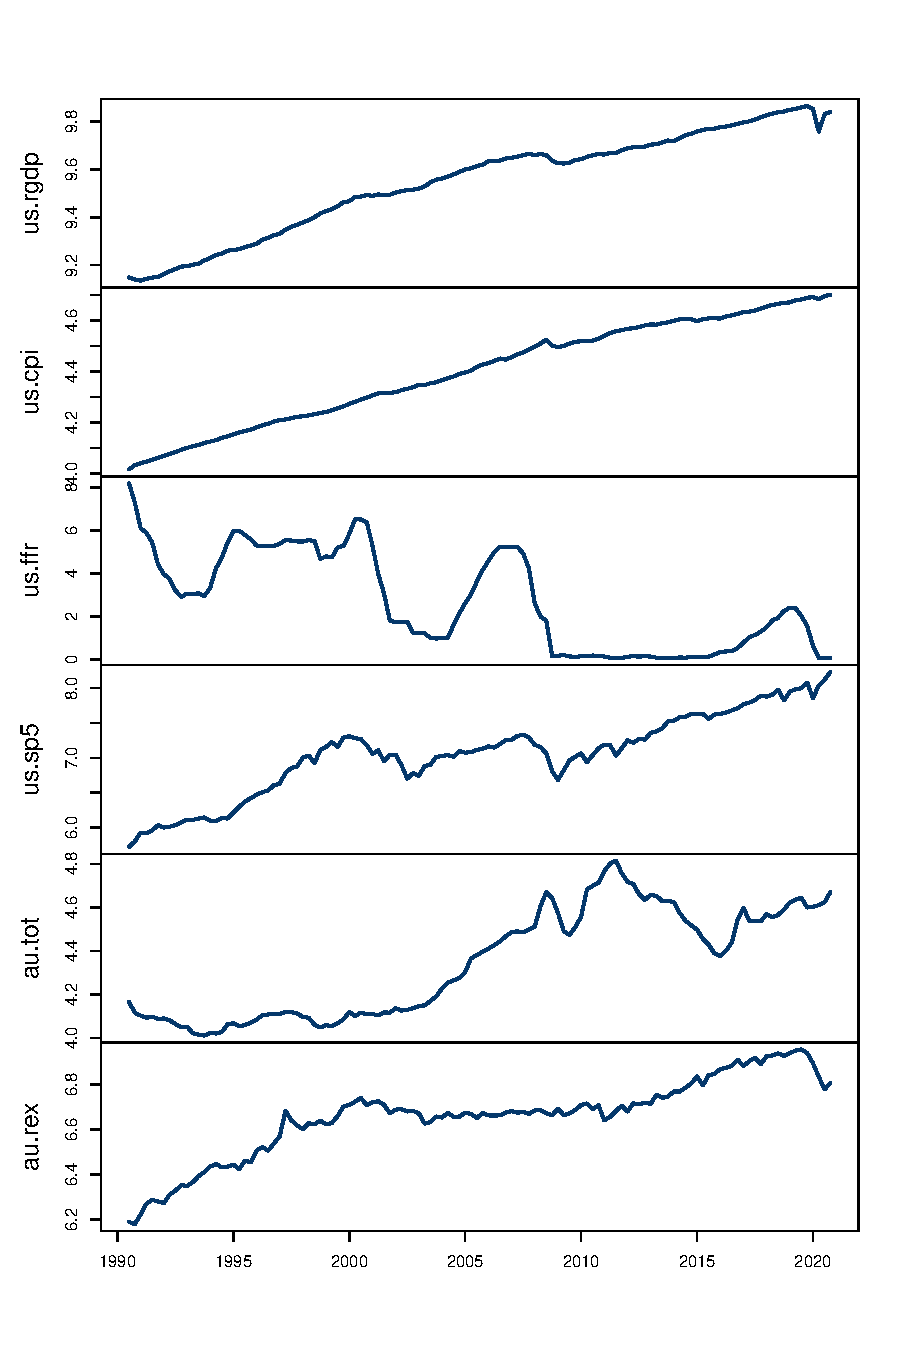
\includegraphics[scale=0.37, trim=1.5cm 0cm 0cm 0cm]{data-foreign.pdf}
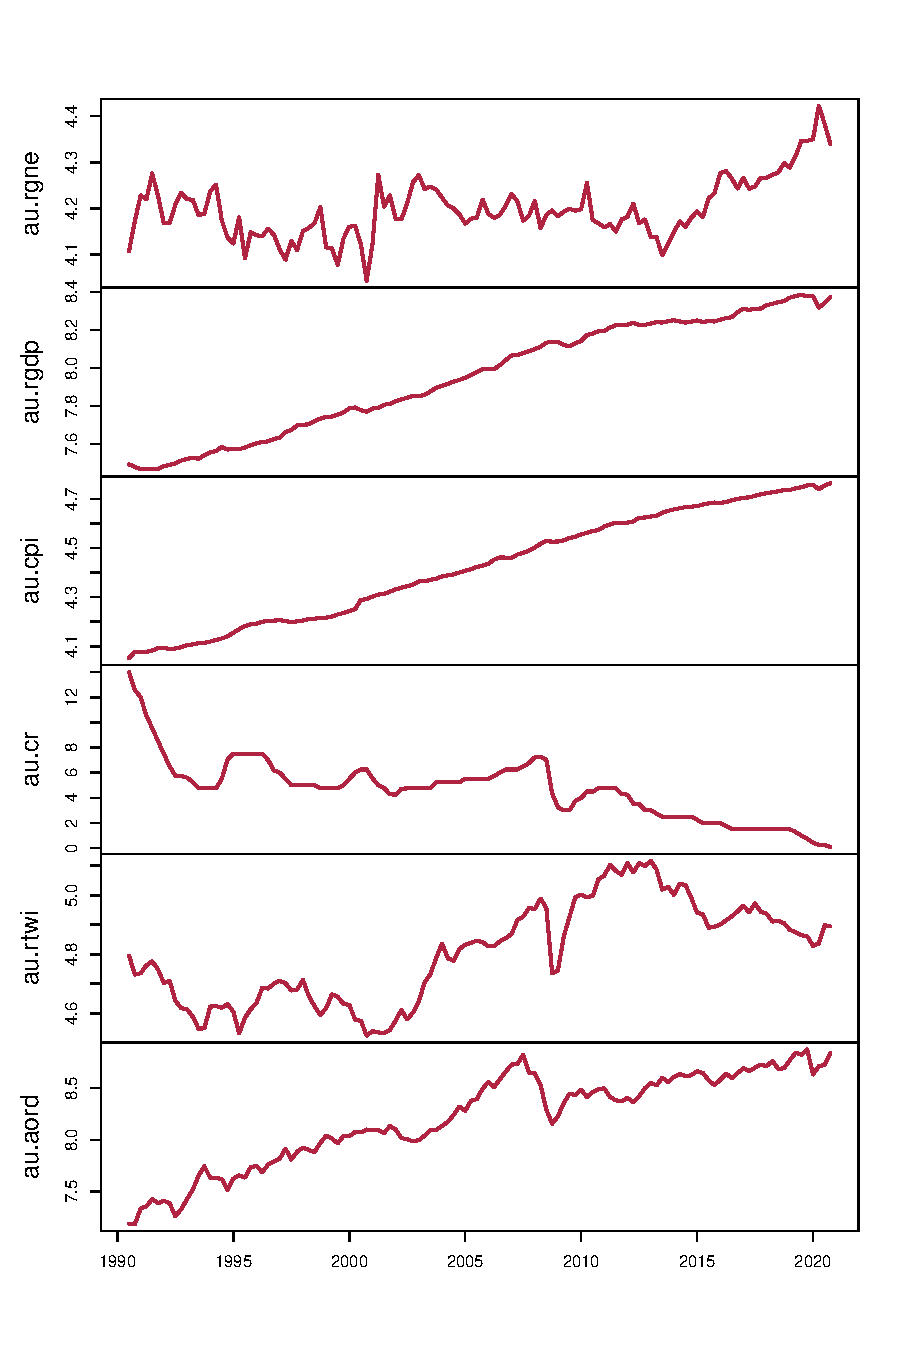
\includegraphics[scale=0.37, trim=0.6cm 0cm 1cm 0cm]{data-domestic.pdf}

\end{frame}
%}


\begin{frame}{SVAR Model of the Australian Economy}
\footnotesize
\begin{align*}
\begin{bmatrix} {\color{mcxs1}B_{0.11}} & {\color{purple}\mathbf{0}_{6\times6}} \\ B_{0.21} & {\color{purple}B_{0.22}} \end{bmatrix}&\begin{bmatrix} {\color{mcxs1}y_t^{f}} \\ {\color{purple}y_t^d} \end{bmatrix} = \begin{bmatrix} {\color{mcxs1}b_{0.1}}\\{\color{purple}b_{0.2}} \end{bmatrix}  + \begin{bmatrix} {\color{mcxs1}B_{1.11}} & {\color{mcxs1}B_{1.12}} \\ B_{1.21} & {\color{purple}B_{1.22}} \end{bmatrix} \begin{bmatrix} {\color{mcxs1}y_{t-1}^{f}} \\ {\color{purple}y_{t-1}^d} \end{bmatrix} + \dots +  \begin{bmatrix} {\color{mcxs1}u_t^{f}} \\ {\color{purple}u_t^d} \end{bmatrix} \\[2ex]
{\color{mcxs1}y_t^{f\prime}} &= \begin{bmatrix} {\color{mcxs1}rgdp_t} & {\color{mcxs1}cpi_t} & {\color{mcxs1}FFR_t} & {\color{mcxs1}sp500_t} & {\color{mcxs1}tot_t} & {\color{mcxs1}rex_t} \end{bmatrix}\\
{\color{purple}y_t^{d\prime}} &= \begin{bmatrix} {\color{purple}rgne_t} & {\color{purple}rgdp_t} & {\color{purple}cpi_t} & {\color{purple}CR_t} & {\color{purple}rtwi_t} & {\color{purple}aord_t} \end{bmatrix}\\
{\color{mcxs1}u_t^{f\prime}} &= \begin{bmatrix} {\color{mcxs1}u_{1.t}} & {\color{mcxs1}u_{2.t}} & {\color{mcxs1}u_{3.t}^{us.mps}} & {\color{mcxs1}u_{4.t}} & {\color{mcxs1}u_{5.t}} & {\color{mcxs1}u_{6.t}} \end{bmatrix}\\
{\color{purple}u_t^{d\prime}} &= \begin{bmatrix} {\color{purple}u_{7.t}} & {\color{purple}u_{8.t}} & {\color{purple}u_{9.t}} & {\color{purple}u_{10.t}^{au.mps}} & {\color{purple}u_{11.t}} & {\color{purple}u_{12.t}} \end{bmatrix}
\end{align*}

\bigskip\textbf{Foreign block.}\\ \scriptsize
${\color{mcxs1}rgdp_t}$ {\color{mcxs2}-- real GDP,}
${\color{mcxs1}cpi_t}$ {\color{mcxs2}-- CPI,}
${\color{mcxs1}FFR_t}$ {\color{mcxs2}-- federal funds rate,}
${\color{mcxs1}sp500_t}$ {\color{mcxs2}-- S\&P 500 index,}
${\color{mcxs1}tot_t}$ {\color{mcxs2}-- Australian terms of trade,}
${\color{mcxs1}rex_t}$ {\color{mcxs2}-- Australian real export}

\footnotesize\bigskip\textbf{Australian block.}\\ \scriptsize
${\color{purple}rgne_t}$ {\color{mcxs2}-- real gross national expenditure,}
${\color{purple}rgdp_t}$ {\color{mcxs2}-- real GDP,}
${\color{purple}cpi_t}$ {\color{mcxs2}-- CPI,}\\
${\color{purple}CR_t}$ {\color{mcxs2}-- cash rate,}
${\color{purple}rtwi_t}$ {\color{mcxs2}-- real trade weighted index,}
${\color{purple}aord_t}$ {\color{mcxs2}-- All Ordinaries Index}

\footnotesize\bigskip\textbf{Shocks of interest.}\\ \scriptsize
${\color{purple}u_{10.t}^{au.mps}}$ {\color{mcxs2}-- Australian monetary policy shock}\\[1ex]
${\color{mcxs1}u_{3.t}^{us.mps}}$ {\color{mcxs2}-- US  monetary policy shock}
\end{frame}



\begin{frame}{SVAR Model of the Australian Economy}

$$
\begin{bmatrix} {\color{mcxs1}B_{0.11}} & {\color{purple}\mathbf{0}_{6\times6}} \\ B_{0.21} & {\color{purple}B_{0.22}} \end{bmatrix}\begin{bmatrix} {\color{mcxs1}y_t^{f}} \\ {\color{purple}y_t^d} \end{bmatrix} = \begin{bmatrix} {\color{mcxs1}b_{0.1}}\\{\color{purple}b_{0.2}} \end{bmatrix}  + \begin{bmatrix} {\color{mcxs1}B_{1.11}} & {\color{mcxs1}B_{1.12}} \\ B_{1.21} & {\color{purple}B_{1.22}} \end{bmatrix} \begin{bmatrix} {\color{mcxs1}y_{t-1}^{f}} \\ {\color{purple}y_{t-1}^d} \end{bmatrix} + \dots +  \begin{bmatrix} {\color{mcxs1}u_t^{f}} \\ {\color{purple}u_t^d} \end{bmatrix}
$$


\bigskip\textbf{SVAR for a small-open economy}
\begin{description}
\item[${\color{mcxs1}B_{0.11}}$] {\color{mcxs2}-- identification of foreign shocks: lower-triangular matrix}
\item[${\color{purple}B_{0.22}}$] {\color{mcxs2}-- identification of domestic shocks: lower-triangular matrix}
\item[${\color{purple}B_{0.12}}={\color{purple}\mathbf{0}_{6\times6}}$] {\color{mcxs2}-- small-open economy assumption}
\item[${\color{purple}B_{l.12}}={\color{purple}\mathbf{0}_{6\times6}}$] {\color{mcxs2}-- small-open economy assumption (not imposed)}
\item[$B_{0.21}$] {\color{mcxs2}-- small-open economy assumption: foreign shocks affect domestic variables}
\end{description}

\end{frame}







\begin{frame}{SVAR Model of the Australian Economy}

$$
\begin{bmatrix} {\color{mcxs1}B_{0.11}} & {\color{purple}\mathbf{0}_{6\times6}} \\ B_{0.21} & {\color{purple}B_{0.22}} \end{bmatrix}\begin{bmatrix} {\color{mcxs1}y_t^{f}} \\ {\color{purple}y_t^d} \end{bmatrix} = \begin{bmatrix} {\color{mcxs1}b_{0.1}}\\{\color{purple}b_{0.2}} \end{bmatrix}  + \begin{bmatrix} {\color{mcxs1}B_{1.11}} & {\color{mcxs1}B_{1.12}} \\ B_{1.21} & {\color{purple}B_{1.22}} \end{bmatrix} \begin{bmatrix} {\color{mcxs1}y_{t-1}^{f}} \\ {\color{purple}y_{t-1}^d} \end{bmatrix} + \dots +  \begin{bmatrix} {\color{mcxs1}u_t^{f}} \\ {\color{purple}u_t^d} \end{bmatrix}
$$


\bigskip\textbf{SVAR for a small-open economy}\small
\begin{itemize}[label=$\blacktriangleright$]
\item The model was estimated using Waggoner \& Zha (2003) algorithm
\item $\underline{B}$ and $\underline{\Omega}$ prior matrices are set the same way as the RF Minnesota prior with $\kappa_1=\kappa_2=1$, $\kappa_3=0.95$
\item $\underline{S}=\kappa_4I_N$ and $\kappa_4=1$, $\underline{\nu}=N$ which make the generalized-normal prior for $B_0$ set to $\mathcal{N}(\mathbf{0}_N,I_N)$
\item The results are sensitive to the specification of $\kappa_1$ and $\kappa_4$
\item The Gibbs sampler for $B_0$ used $S_1=100$ draws in the burin-in and $S_2=5000$ in the final sampler
\item The potential extensions include: estimation of prior hyper-parameters and heteroskedasticity of the structural shocks
\end{itemize}

\end{frame}


\begin{frame}{IRFs of domestic sector to $u_{10.t}^{au.mps}$}
\centering
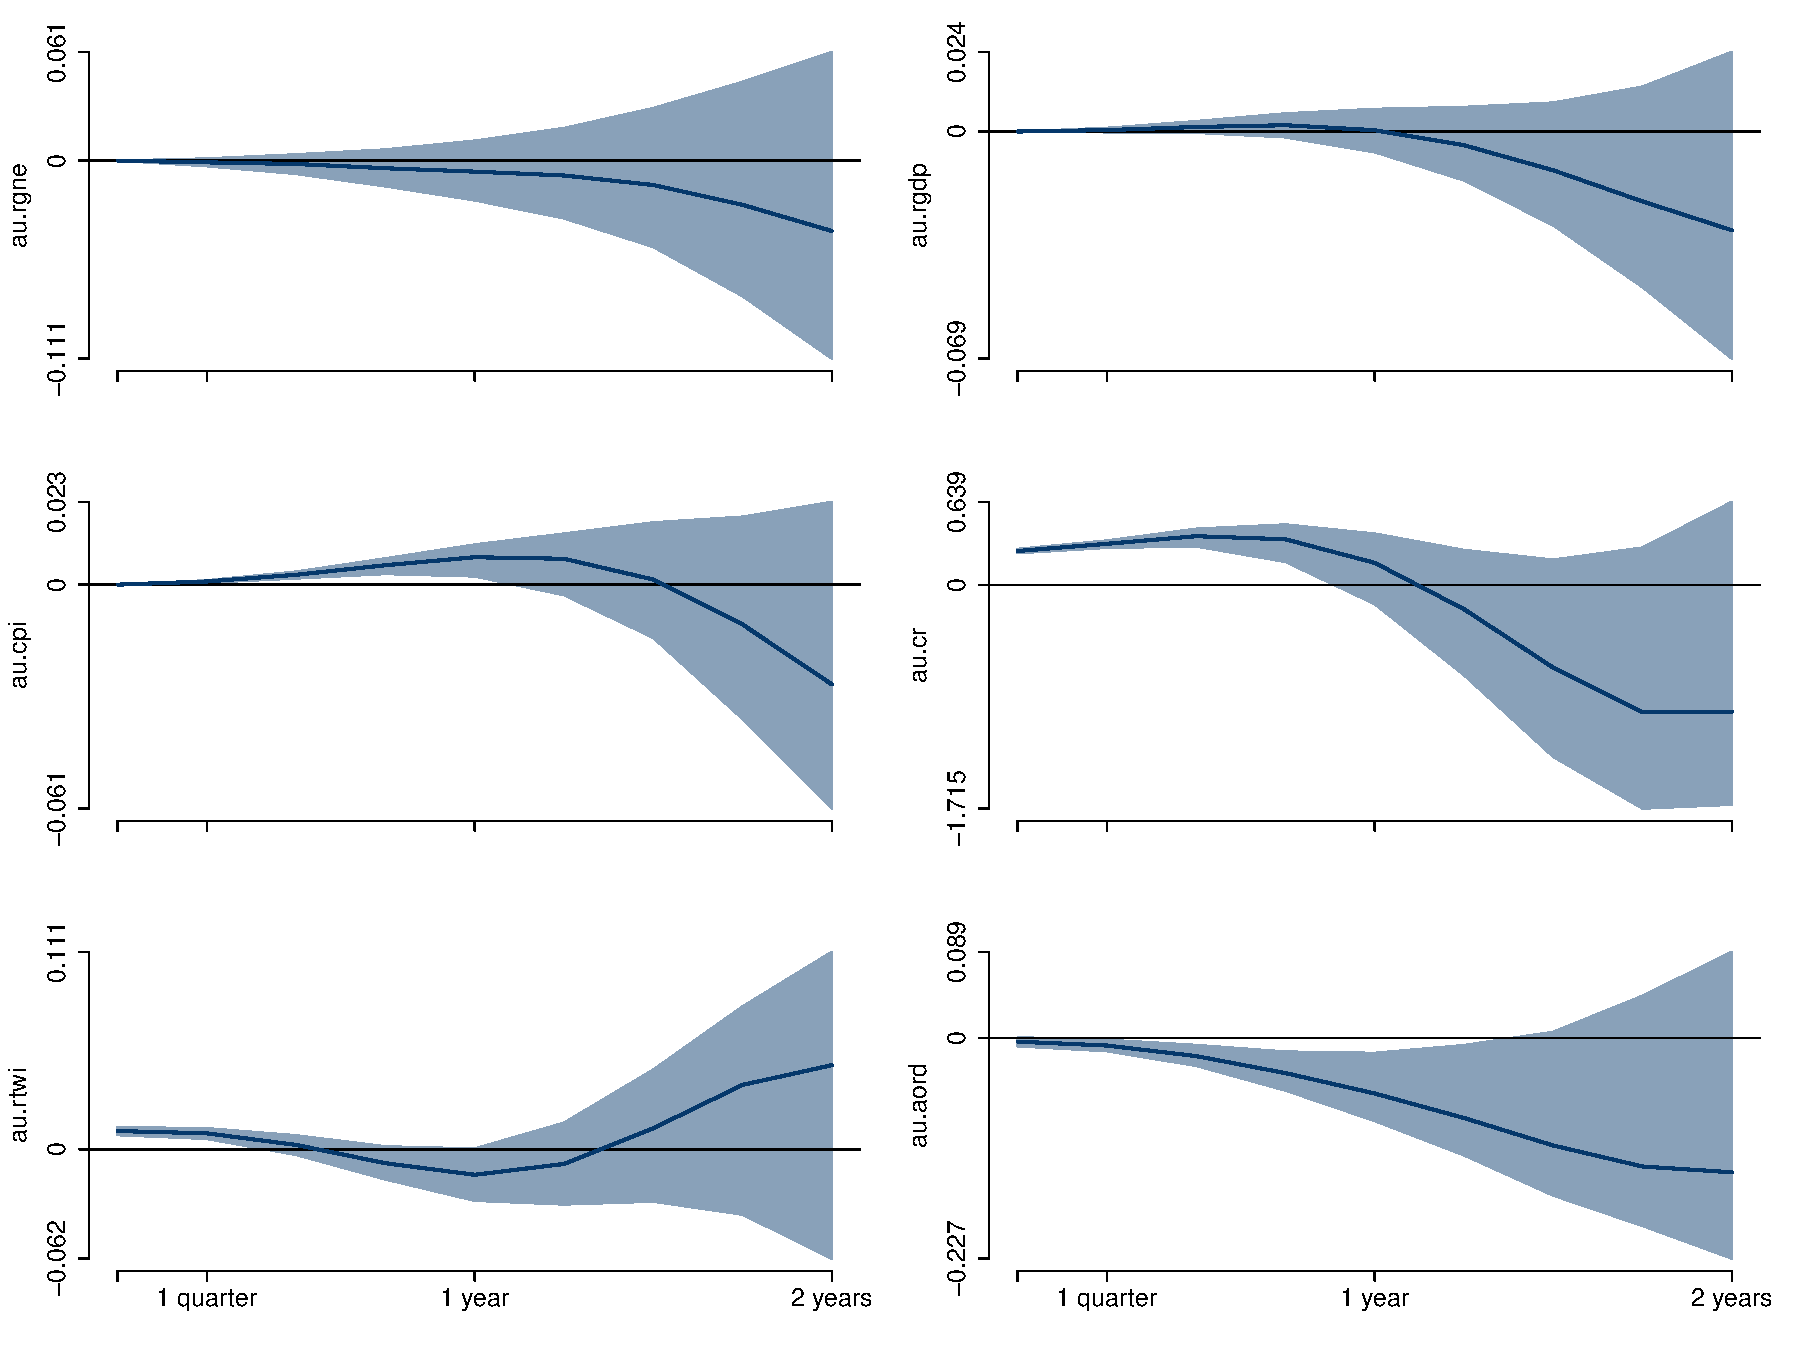
\includegraphics[scale=0.35]{irf-au-mps.pdf}

\end{frame}

\begin{frame}{IRFs of domestic sector to $u_{3.t}^{us.mps}$}
\centering
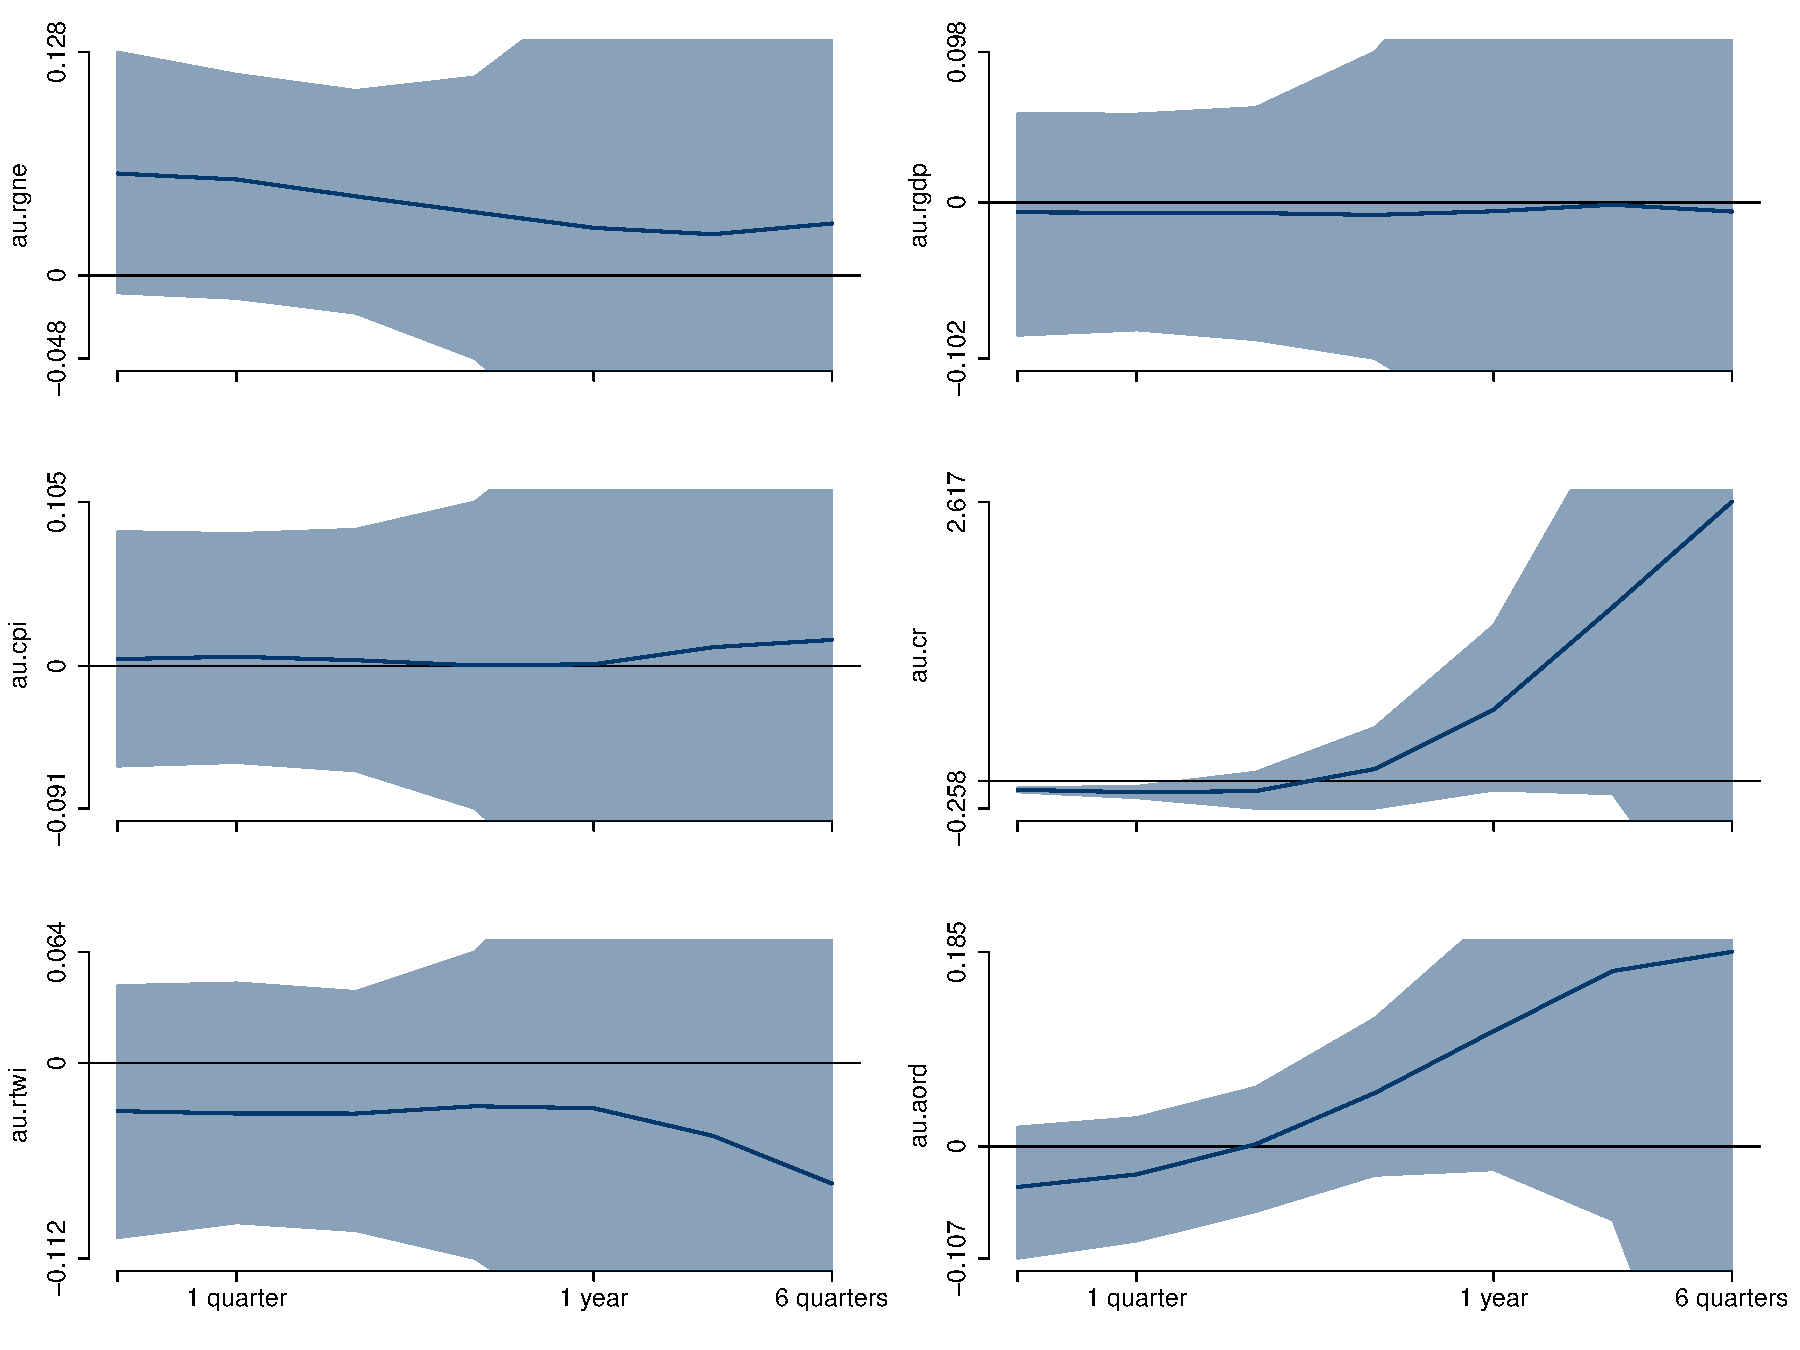
\includegraphics[scale=0.35]{irf-us-mps.pdf}

\end{frame}


\begin{frame}{Forecast error variance decomposition of $au.cpi_{t+h|t}$}

\centering
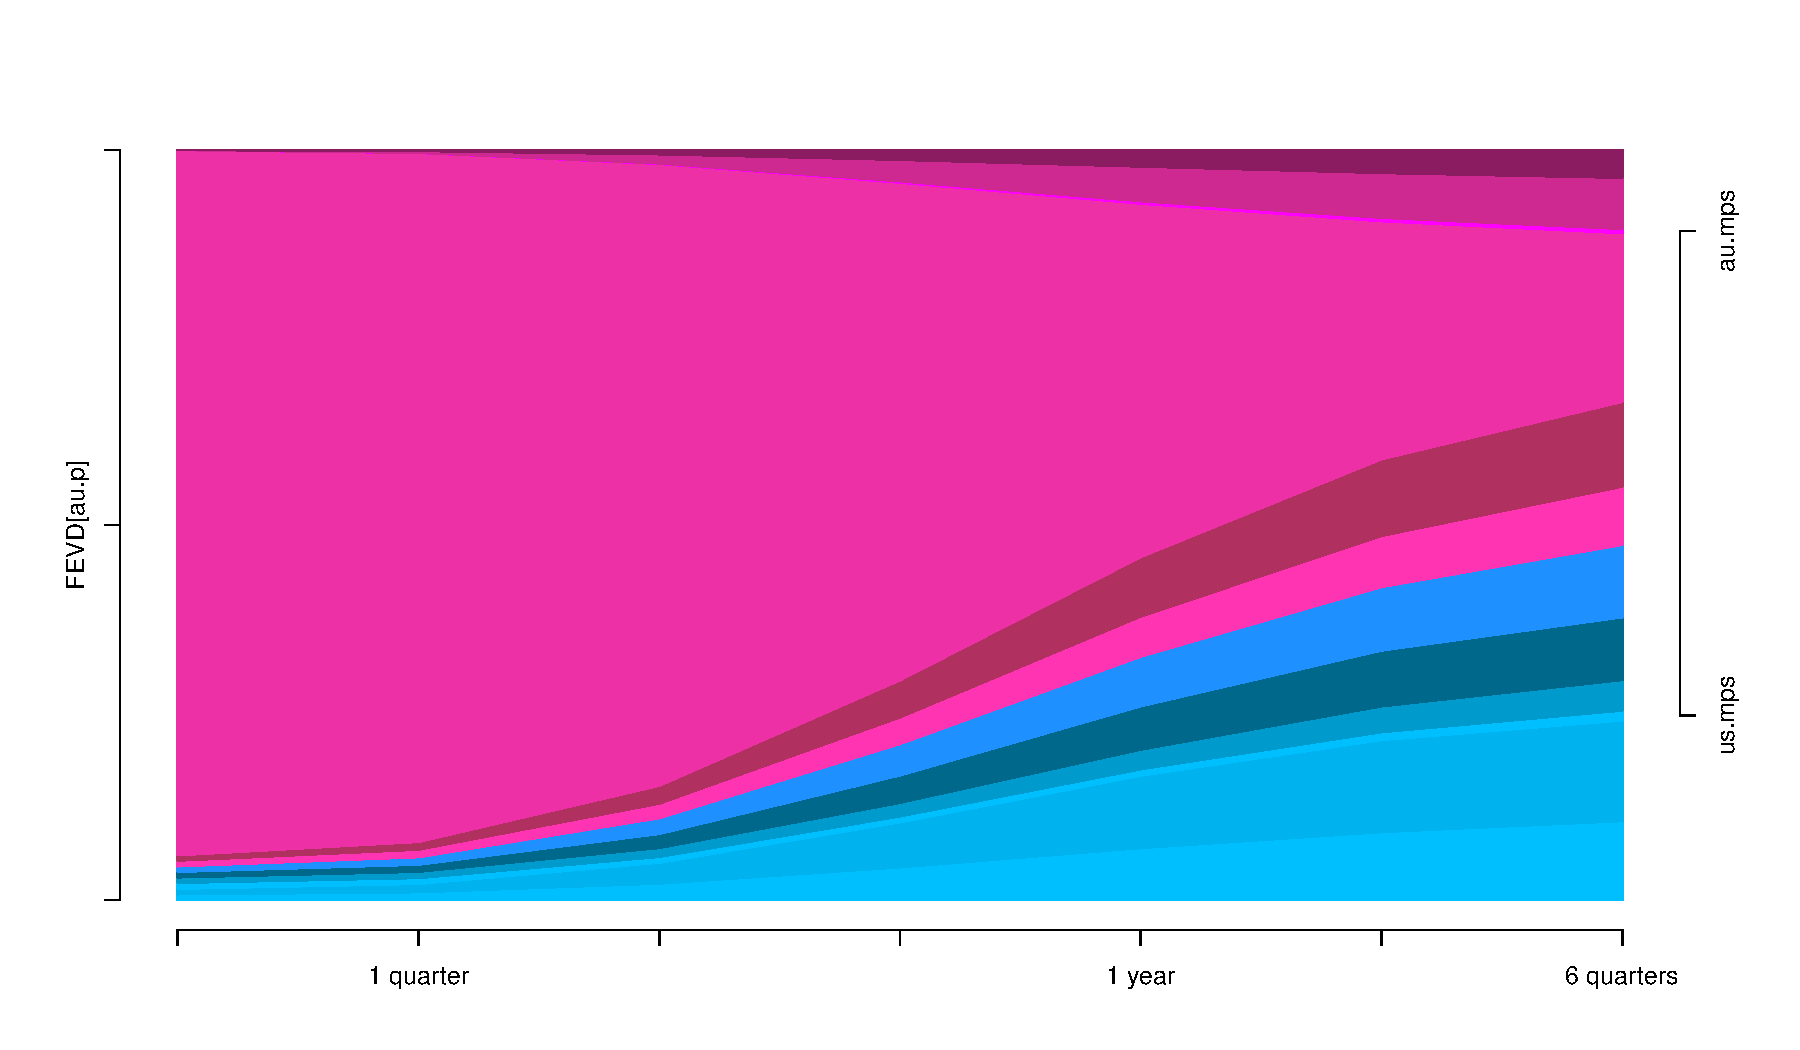
\includegraphics[scale=0.36]{fevd-au-p}

\end{frame}


\begin{frame}{Forecast error variance decomposition of $au.rgdp_{t+h|t}$}

\centering
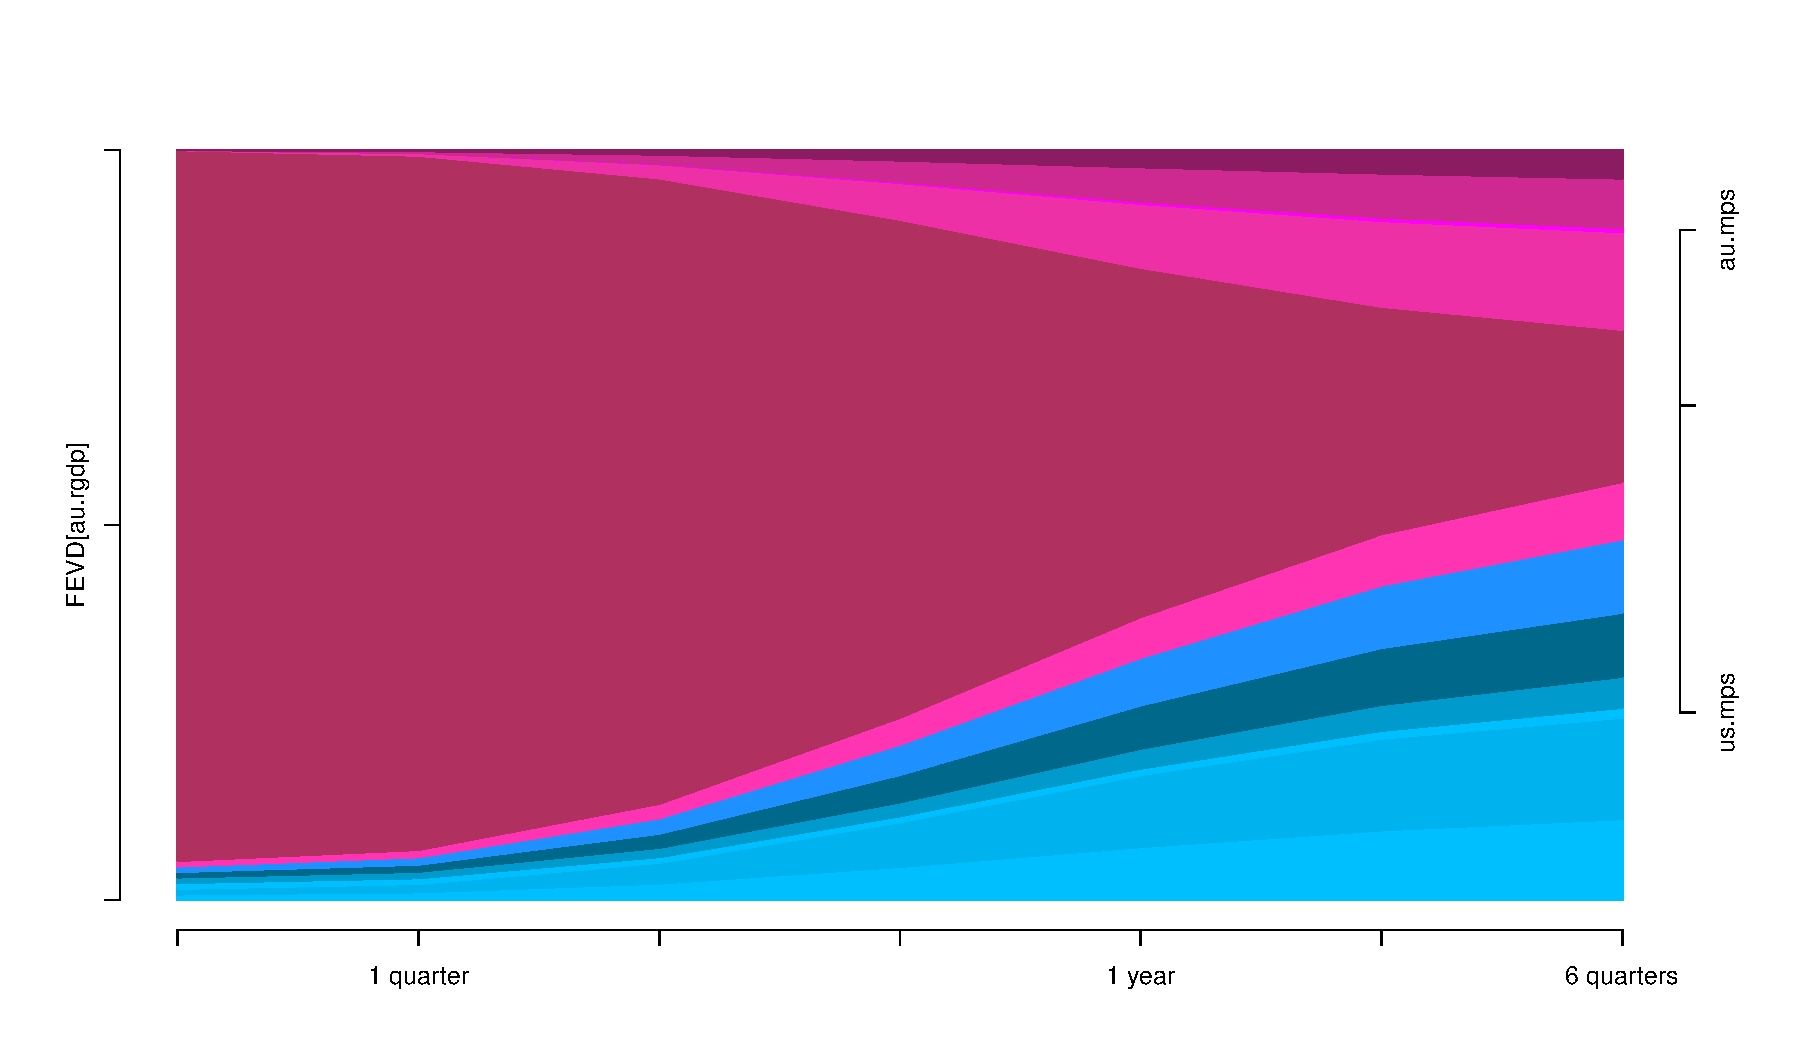
\includegraphics[scale=0.36]{fevd-au-gdp}

\end{frame}



















\begin{frame}{SVAR Model of the Australian Economy}

\begin{align*}
\begin{bmatrix} {\color{mcxs1}B_{0.11}} & {\color{purple}\mathbf{0}_{6\times6}} \\ B_{0.21} & {\color{purple}B_{0.22}} \end{bmatrix}&\begin{bmatrix} {\color{mcxs1}y_t^{f}} \\ {\color{purple}y_t^d} \end{bmatrix} = \begin{bmatrix} {\color{mcxs1}b_{0.1}}\\{\color{purple}b_{0.2}} \end{bmatrix}  + \begin{bmatrix} {\color{mcxs1}B_{1.11}} & {\color{mcxs1}B_{1.12}} \\ B_{1.21} & {\color{purple}B_{1.22}} \end{bmatrix} \begin{bmatrix} {\color{mcxs1}y_{t-1}^{f}} \\ {\color{purple}y_{t-1}^d} \end{bmatrix} + \dots +  \begin{bmatrix} {\color{mcxs1}u_t^{f}} \\ {\color{purple}u_t^d} \end{bmatrix} \\[2ex]
{\color{mcxs1}y_t^{f\prime}} &= \begin{bmatrix} {\color{mcxs1}rgdp_t} & {\color{mcxs1}cpi_t} & {\color{mcxs1}FFR_t} & {\color{mcxs1}sp500_t} & {\color{mcxs1}tot_t} & {\color{mcxs1}rex_t} \end{bmatrix}\\
{\color{purple}y_t^{d\prime}} &= \begin{bmatrix} {\color{purple}rgne_t} & {\color{purple}rgdp_t} & {\color{purple}cpi_t} & {\color{purple}CR_t} & {\color{purple}rtwi_t} & {\color{purple}aord_t} \end{bmatrix}
\end{align*}

\textbf{Shocks of interest.}\\
$u_{t}^{f}$ -- foreign shocks\\[1ex]
${\color{purple}u_{t}^{d}}$ {\color{purple}-- domestic shocks}

\bigskip\textbf{Objective.}\\
To identify to what extent the foreign shocks determine the business cycle in Australia jointly
\end{frame}



\begin{frame}{SVAR Model of the Australian Economy}

$$
\begin{bmatrix} {\color{mcxs1}B_{0.11}} & {\color{purple}\mathbf{0}_{6\times6}} \\ B_{0.21} & {\color{purple}B_{0.22}} \end{bmatrix}\begin{bmatrix} {\color{mcxs1}y_t^{f}} \\ {\color{purple}y_t^d} \end{bmatrix} = \begin{bmatrix} {\color{mcxs1}b_{0.1}}\\{\color{purple}b_{0.2}} \end{bmatrix}  + \begin{bmatrix} {\color{mcxs1}B_{1.11}} & {\color{mcxs1}B_{1.12}} \\ B_{1.21} & {\color{purple}B_{1.22}} \end{bmatrix} \begin{bmatrix} {\color{mcxs1}y_{t-1}^{f}} \\ {\color{purple}y_{t-1}^d} \end{bmatrix} + \dots +  \begin{bmatrix} {\color{mcxs1}u_t^{f}} \\ {\color{purple}u_t^d} \end{bmatrix}
$$
\textbf{SVAR for a small-open economy.}\small
\begin{description}
\item[$B_{11}, {\color{purple}B_{22}}$] {\color{purple}-- unrestricted}
\item[${\color{purple}B_{12}}={\color{purple}\mathbf{0}_{6\times6}}$] {\color{mcxs1}-- small-open economy assumption}
\item[$B_{0.21}$] -- small-open economy assumption: unrestricted
\end{description}

\bigskip\normalsize\textbf{Identification.}\\ \small
The model is identified up to a block diagonal rotation matrix
$$ Q = \begin{bmatrix} Q_1 & \mathbf{0}_{6\times 6}\\ \mathbf{0}_{6\times 6} & Q_2\end{bmatrix} $$
\begin{description}
\item[$Q_1$, $Q_2$] {\color{mcxs2}-- $6\times 6$ rotation matrices (drawn from Haar distribution)}
\end{description}

\smallskip The model has been estimated by premultiplying every draw of matrices $B_0$ and $B_+$ by the corresponding draw of matrix $Q$

\end{frame}





\begin{frame}{Forecast error variance decomposition of $au.cpi_{t+h|t}$}

\centering
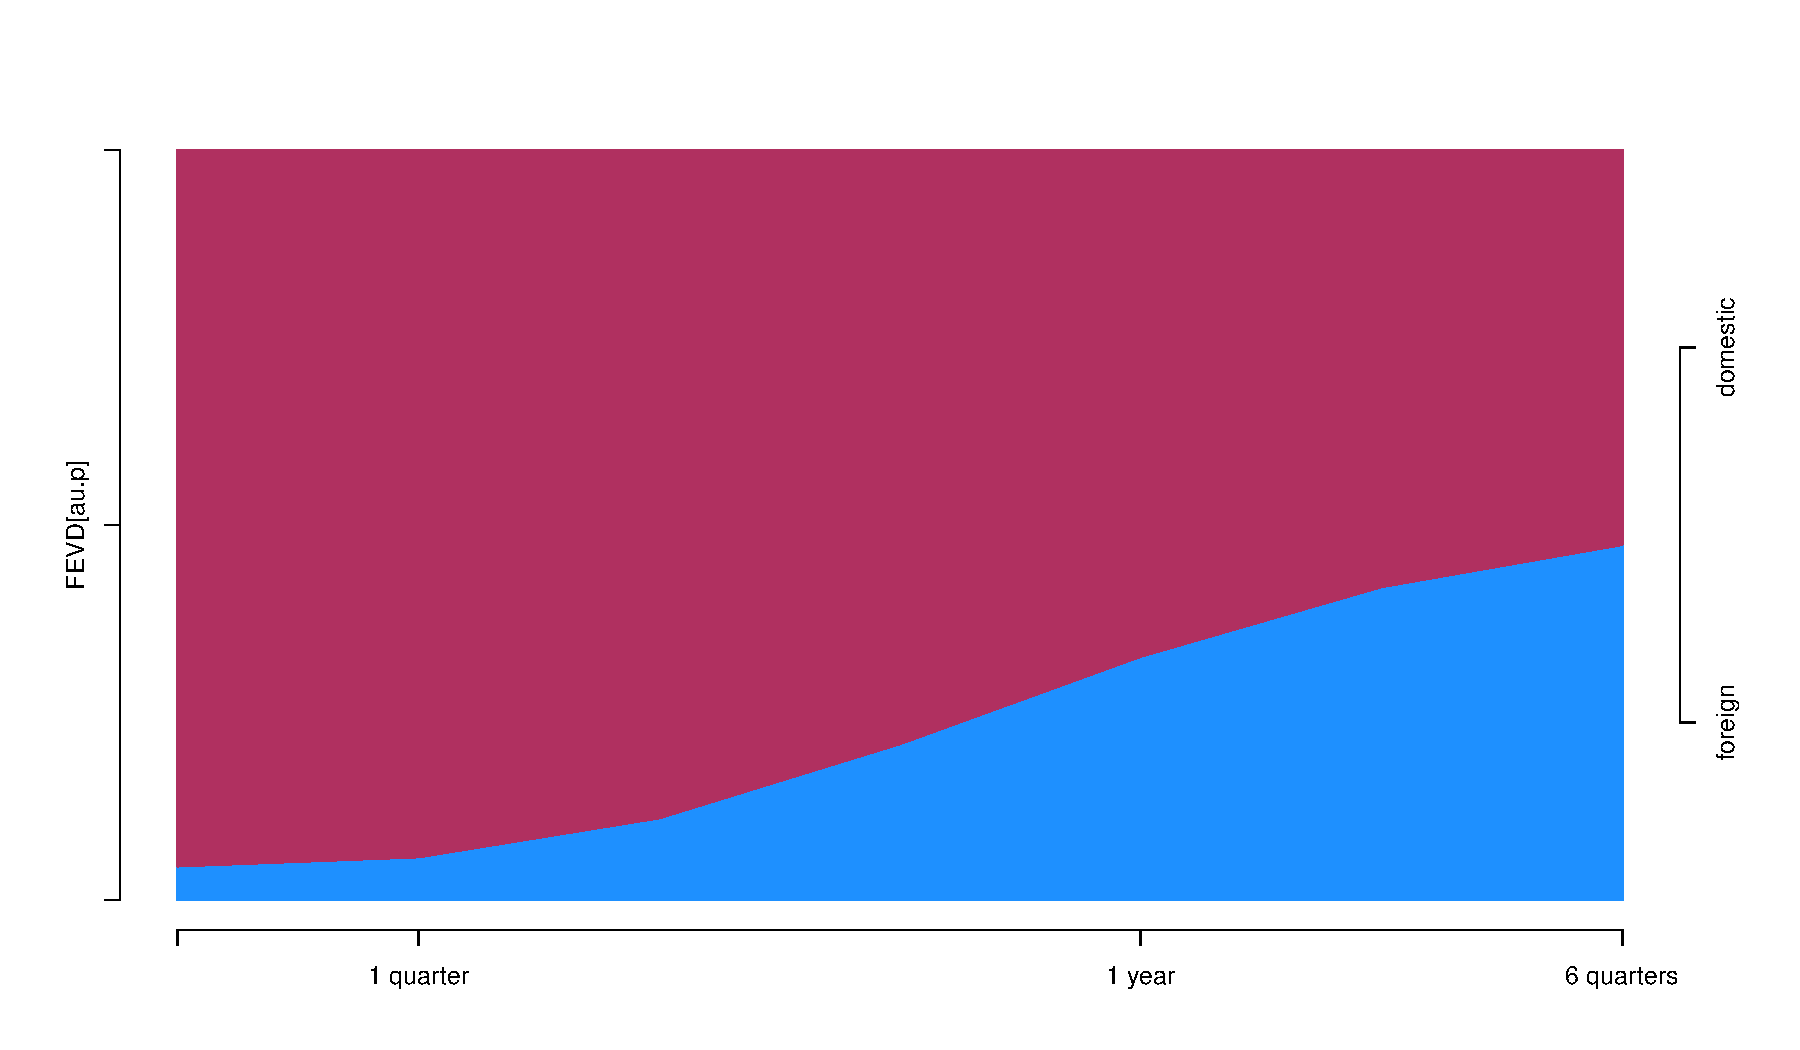
\includegraphics[scale=0.36]{fevd-au-fd-p}

\end{frame}


\begin{frame}{Forecast error variance decomposition of $au.rgdp_{t+h|t}$}

\centering
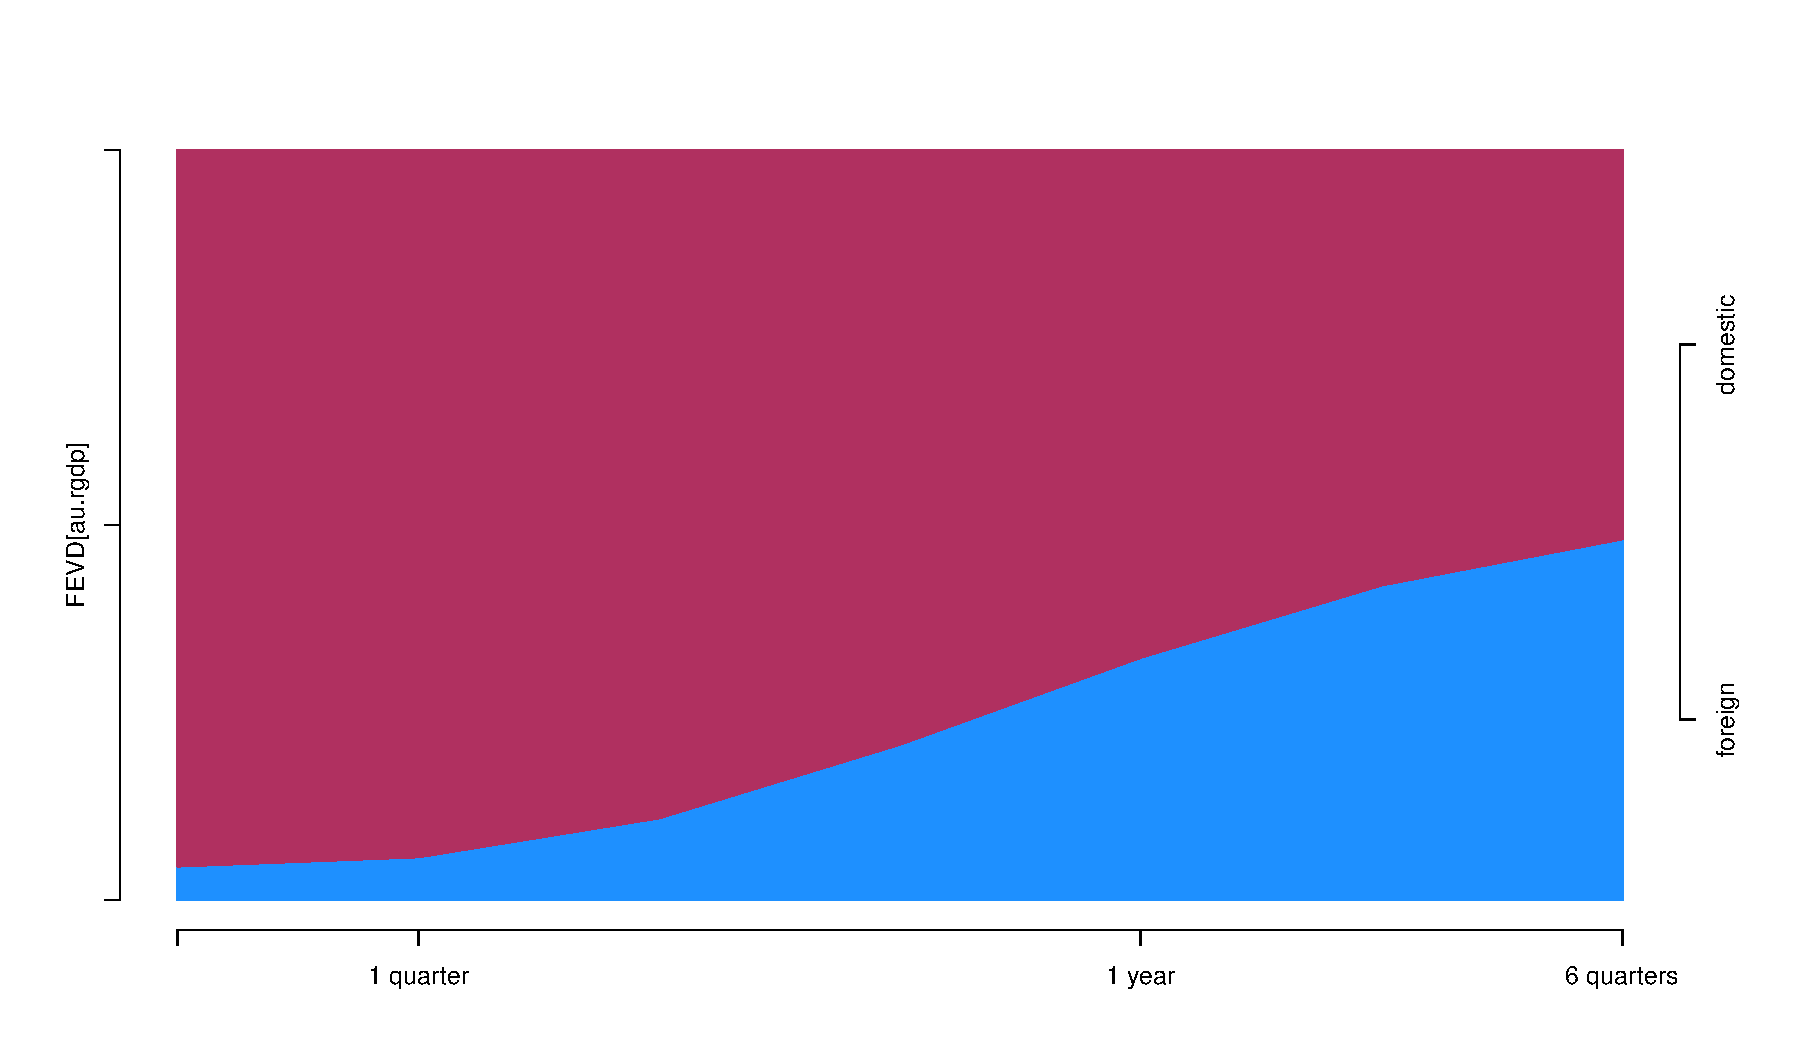
\includegraphics[scale=0.36]{fevd-au-fd-gdp}

\end{frame}















{\setbeamercolor{background canvas}{bg=mcxs1}
\begin{frame}

\begin{center}
\vspace{1cm}\Large\textbf{\color{purple}Modeling effects of monetary policy in the US}%\\ \textbf{\color{mcxs2} Basic analysis}
\end{center}

\end{frame}
}


\begin{frame}{Modeling effects of monetary policy: {\color{purple}data}}

\centering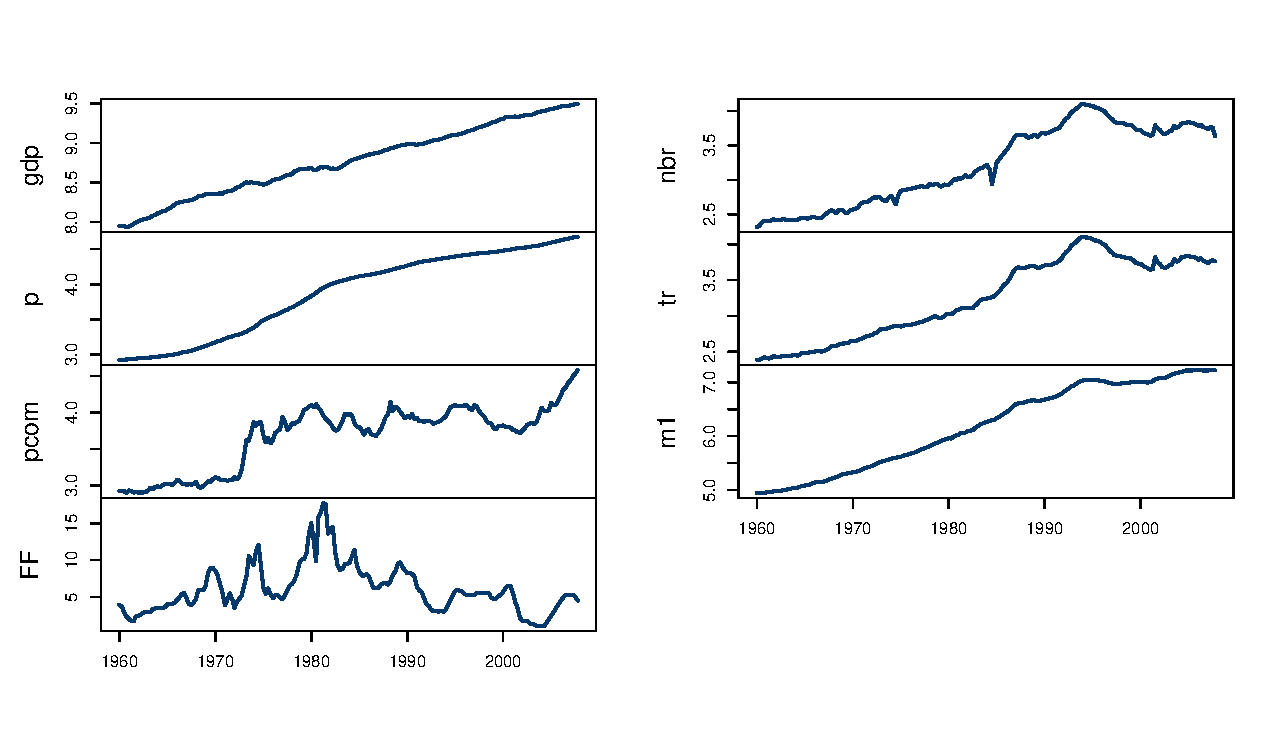
\includegraphics[scale=0.55, trim=1cm 1cm 0cm 0cm]{data-us.pdf}

\begin{center}
\small {\color{mcxs2}Quarterly data from 1961 Q2 to 2007 Q4.} 
\end{center}

\smallskip\scriptsize $  rgdp_t$ {\color{mcxs2}-- real GDP,} $  p_t$ {\color{mcxs2}-- GDP price deflator,} $  pcom_t$ {\color{mcxs2}-- commodity price index,}\\ $FF_t$ {\color{mcxs2}-- federal funds rate,} $  nbr_t$ {\color{mcxs2}-- non-borrowed reserves,} $  tr_t$ {\color{mcxs2}-- total reserves,}\\  $  m_t$ {\color{mcxs2}-- monetary aggregate M1}

\end{frame}



\begin{frame}{Modeling effects of monetary policy: {\color{purple}models}}

\begin{align*}
{\color{purple}B_0} y_{t} &= b_0 + B_1 y_{t-1} + \dots + B_p y_{t-p} + u_t\\[1ex]
u_t|s_t &\sim \mathcal{N}\left( \mathbf{0}_N, {\color{purple}I_N} \right)
\end{align*}

\bigskip\textbf{SVAR for a small-open economy}\small
\begin{itemize}[label=$\blacktriangleright$]
\item The model was estimated using Waggoner \& Zha (2003) algorithm
\item $\underline{B}$ and $\underline{\Omega}$ prior matrices are set the same way as the RF Minnesota prior with $\kappa_1= 0.1$, $\kappa_2=10$, and $\kappa_3=1$
\item $\underline{S}=\kappa_4I_N$ and $\kappa_4=10$, $\underline{\nu}=N$ which make the generalized-normal prior for $B_0$ set to $\mathcal{N}(\mathbf{0}_N,10 I_N)$
\item The results are sensitive to the specification of $\kappa_1$ and $\kappa_4$
\item The Gibbs sampler for $B_0$ used $S_1=100$ draws in the burin-in and $S_2=5000$ in the final sampler
\item The potential extensions include: estimation of prior hyper-parameters and heteroskedasticity of the structural shocks
\end{itemize}

\end{frame}










\begin{frame}{Modeling effects of monetary policy: {\color{purple}models}}

\textbf{FF policy shock}
{\footnotesize \color{mcxs2}by Bernanke \& Blinder (1992, AER), Sims (1992, EER)}
\begin{equation*}
\begin{bmatrix} 
a_{11} &0&0&0&0&0&0 \\ 
a_{21} &a_{22}&0&0&0&0&0 \\ 
a_{31} &a_{32}&a_{33}&0&0&0&0 \\ 
\color{purple}a_{41} &\color{purple}a_{42}&\color{purple}a_{43}&\color{purple}a_{44}&\color{purple}0&\color{purple}0&\color{purple}0 \\ 
a_{51} &a_{52}&a_{53}&\color{mcxs2}a_{54}&\color{mcxs2}a_{55}&\color{mcxs2}0&0 \\ 
a_{61} &a_{62}&a_{63}&\color{mcxs2}a_{64}&\color{mcxs2}a_{65}&\color{mcxs2}a_{66}&0 \\ 
a_{71} &a_{72}&a_{73}&a_{74}&a_{75}&a_{76}&a_{77} 
\end{bmatrix}
\begin{bmatrix}   rgdp_t \\   p_t \\   pcom_t \\ {\color{purple}FF_t} \\   nbr_t \\   tr_t \\   m_t \end{bmatrix}
\end{equation*}
\end{frame}

\begin{frame}{Modeling effects of monetary policy: {\color{purple}models}}

\textbf{NBR policy shock}
{\footnotesize \color{mcxs2}by Christiano \& Eichenbaum (1992)}
\begin{equation*}
\begin{bmatrix} 
a_{11} &0&0&0&0&0&0 \\ 
a_{21} &a_{22}&0&0&0&0&0 \\ 
a_{31} &a_{32}&a_{33}&0&0&0&0 \\ 
a_{41} &a_{42}&a_{43}&\color{mcxs2}a_{44}&\color{mcxs2}a_{45}&\color{mcxs2}0&0 \\ 
\color{purple}a_{51} &\color{purple}a_{52}&\color{purple}a_{53}&\color{purple}0&\color{purple}a_{55}&\color{purple}0&\color{purple}0 \\ 
a_{61} &a_{62}&a_{63}&\color{mcxs2}a_{64}&\color{mcxs2}a_{65}&\color{mcxs2}a_{66}&0 \\ 
a_{71} &a_{72}&a_{73}&a_{74}&a_{75}&a_{76}&a_{77} 
\end{bmatrix}
\begin{bmatrix}   rgdp_t \\   p_t \\   pcom_t \\ FF_t \\ {\color{purple}  nbr_t} \\   tr_t \\   m_t \end{bmatrix}
\end{equation*}
\end{frame}

\begin{frame}{Modeling effects of monetary policy: {\color{purple}models}}

\textbf{NBR/TR policy shock}
{\footnotesize \color{mcxs2}by Strongin (1995, JME)}
\begin{equation*}
\begin{bmatrix} 
a_{11} &0&0&0&0&0&0 \\ 
a_{21} &a_{22}&0&0&0&0&0 \\ 
a_{31} &a_{32}&a_{33}&0&0&0&0 \\ 
a_{41} &a_{42}&a_{43}&\color{mcxs2}a_{44}&\color{mcxs2}a_{45}&\color{mcxs2}a_{46}&0 \\ 
\color{purple}a_{51} &\color{purple}a_{52}&\color{purple}a_{53}&\color{purple}0&\color{purple}a_{55}&\color{purple}a_{56}&\color{purple}0 \\ 
a_{61} &a_{62}&a_{63}&\color{mcxs2}0&\color{mcxs2}0&\color{mcxs2}a_{66}&0 \\ 
a_{71} &a_{72}&a_{73}&a_{74}&a_{75}&a_{76}&a_{77} 
\end{bmatrix}
\begin{bmatrix}   rgdp_t \\   p_t \\   pcom_t \\ FF_t \\ {\color{purple}  nbr_t} \\   tr_t \\   m_t \end{bmatrix}
\end{equation*}
\end{frame}



%\begin{frame}{Modeling effects of monetary policy: {\color{purple}models}}
%
%\textbf{Sign Restricted policy shock}
%{\footnotesize \color{mcxs2}by Uhlig (2005, JME)}
%\begin{equation*}
%\begin{bmatrix}   rgdp_t \\   p_t \\   pcom_t \\ FF_t \\   nbr_t \\   tr_t \\   m_t \end{bmatrix}\qquad \Theta_i=
%\begin{bmatrix} 
%*&*&*&*&*&*&*\\
%-&*&*&*&*&*&*\\
%-&*&*&*&*&*&*\\
%+&*&*&*&*&*&*\\
%-&*&*&*&*&*&*\\
%-&*&*&*&*&*&*\\
%*&*&*&*&*&*&*\\
%\end{bmatrix}
%\begin{bmatrix} {\color{purple}mps_t} \\ u_{2.t} \\ u_{3.t} \\ u_{4.t} \\ u_{5.t} \\ u_{6.t} \\ u_{7.t} \end{bmatrix}
%\end{equation*}
%
%\smallskip {\color{mcxs2}A monetary policy impulse vector is an impulse vector} $u$ {\color{mcxs2}so that the} {\color{purple}impulse responses} {\color{mcxs2}to} $u$ {\color{mcxs2}of} {\color{purple}prices and non-borrowed reserves are not positive} {\color{mcxs2}and the} {\color{purple}impulse responses for the federal funds rate are not negative}{\color{mcxs2}, all at horizons} $i=0,1,\dots,5$.
%
%\end{frame}



\begin{frame}{Modeling effects of monetary policy: {\color{purple}models}}

\textbf{FF policy shock}
{\footnotesize \color{mcxs2}by Bernanke \& Blinder (1992, AER), Sims (1992, EER)}

\centering
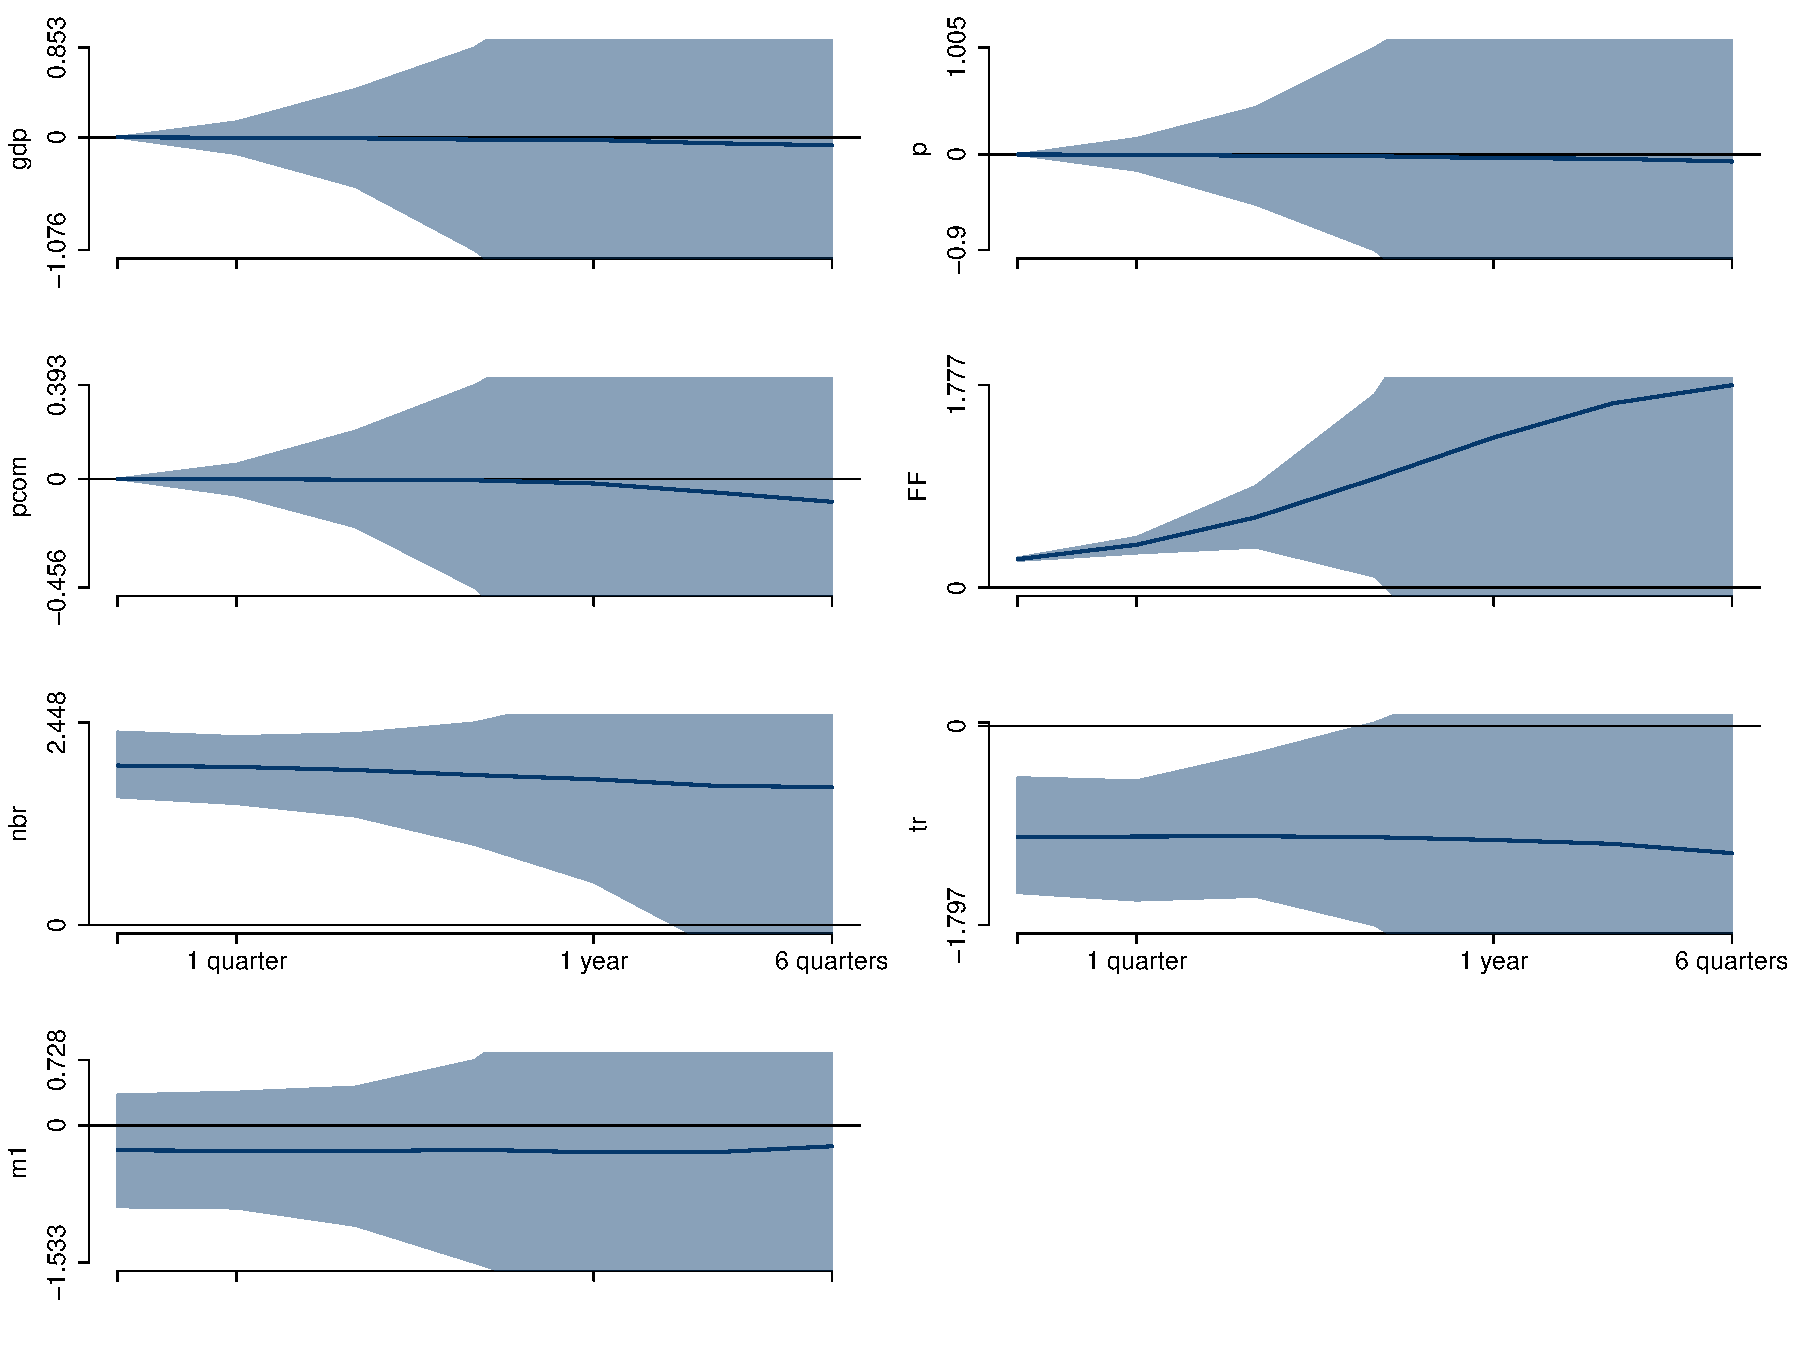
\includegraphics[scale=0.35]{FF-irf-mps.pdf}

\end{frame}



\begin{frame}{Modeling effects of monetary policy: {\color{purple}models}}

\textbf{NBR policy shock}
{\footnotesize \color{mcxs2}by Christiano \& Eichenbaum (1992)}

\centering
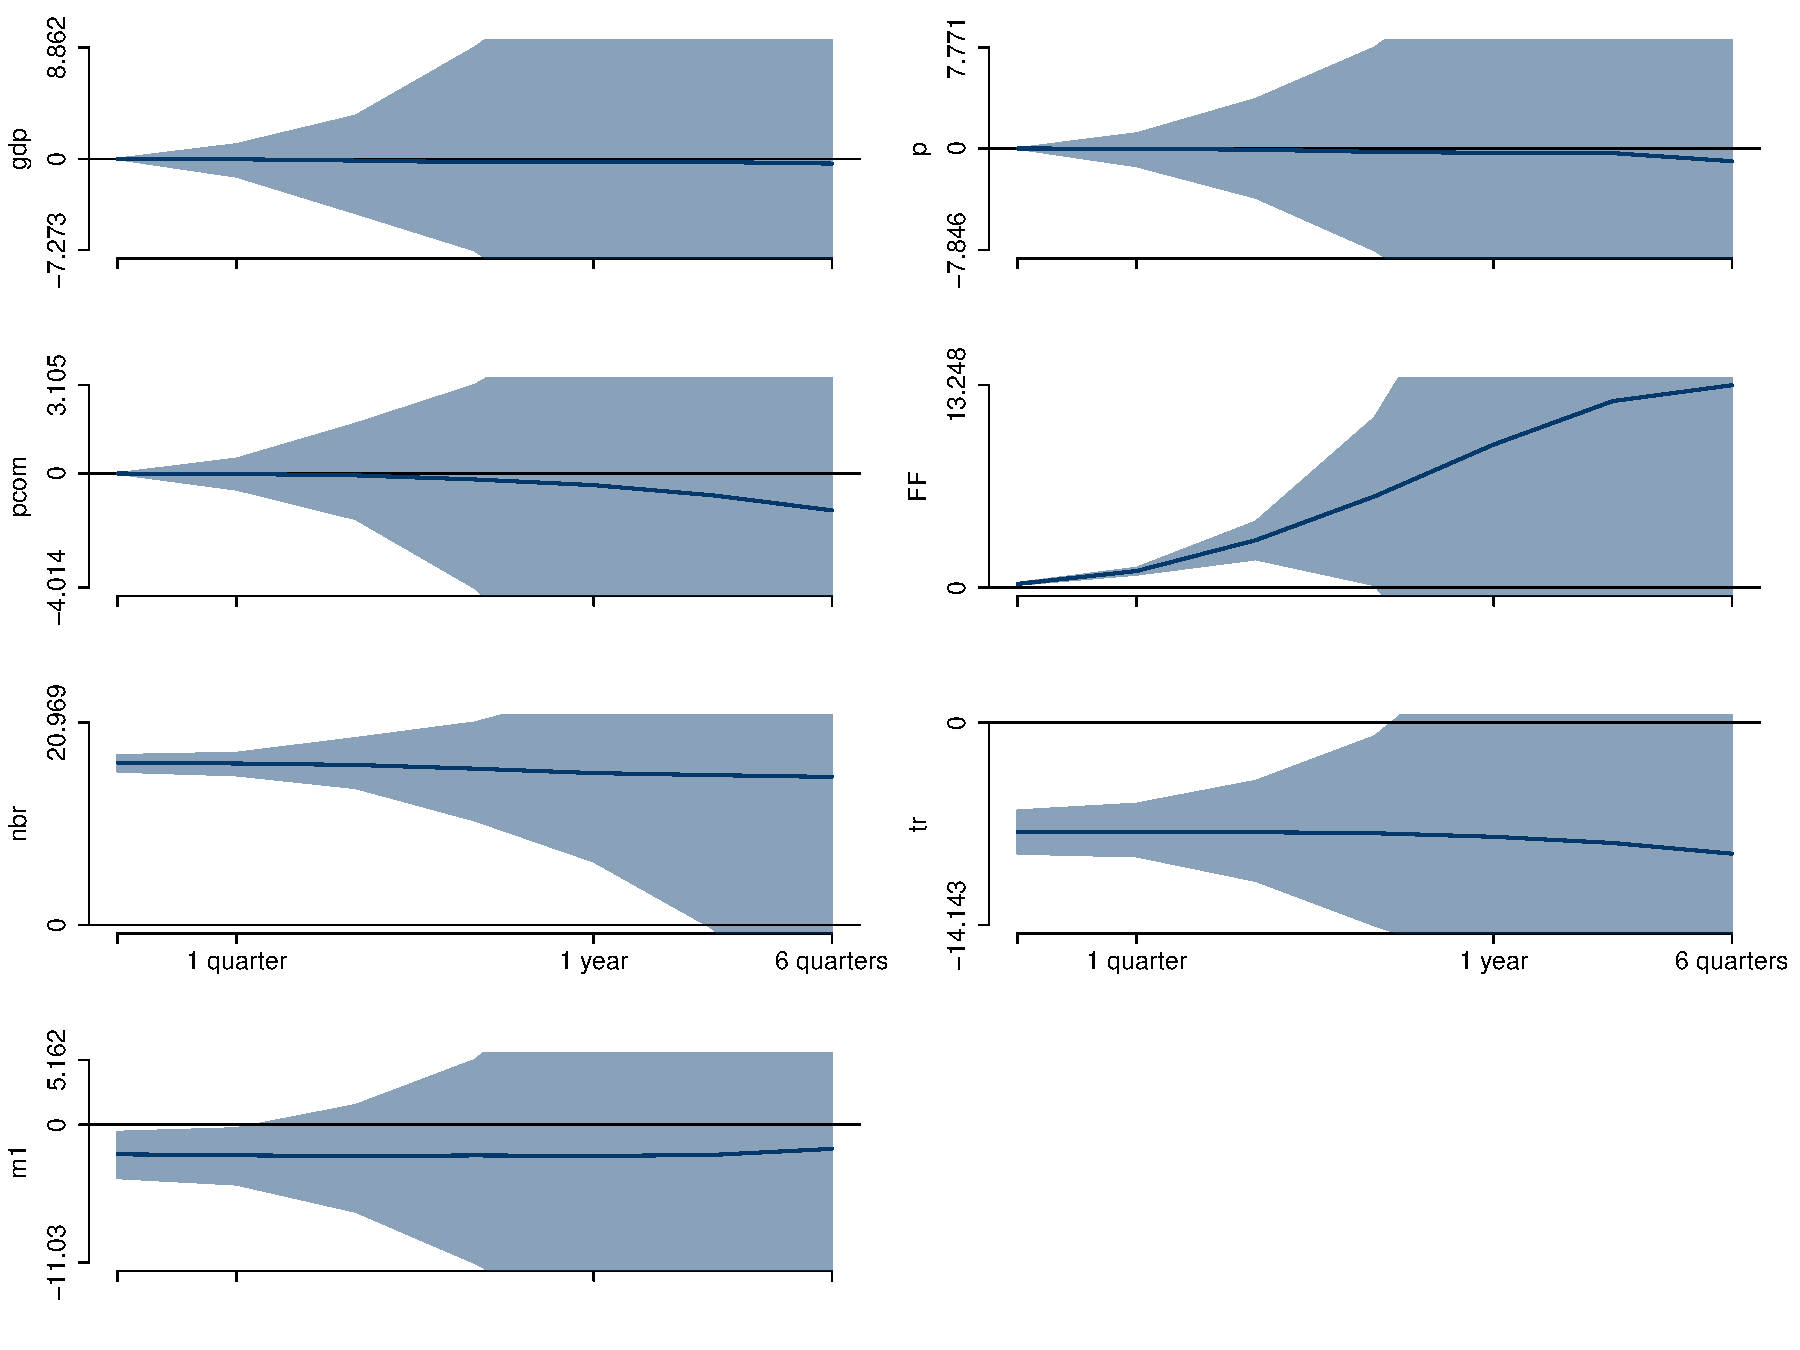
\includegraphics[scale=0.35]{NBR-irf-mps.pdf}

\end{frame}




\begin{frame}{Modeling effects of monetary policy: {\color{purple}models}}

\textbf{NBR/TR policy shock}
{\footnotesize \color{mcxs2}by Strongin (1995, JME)}

\centering
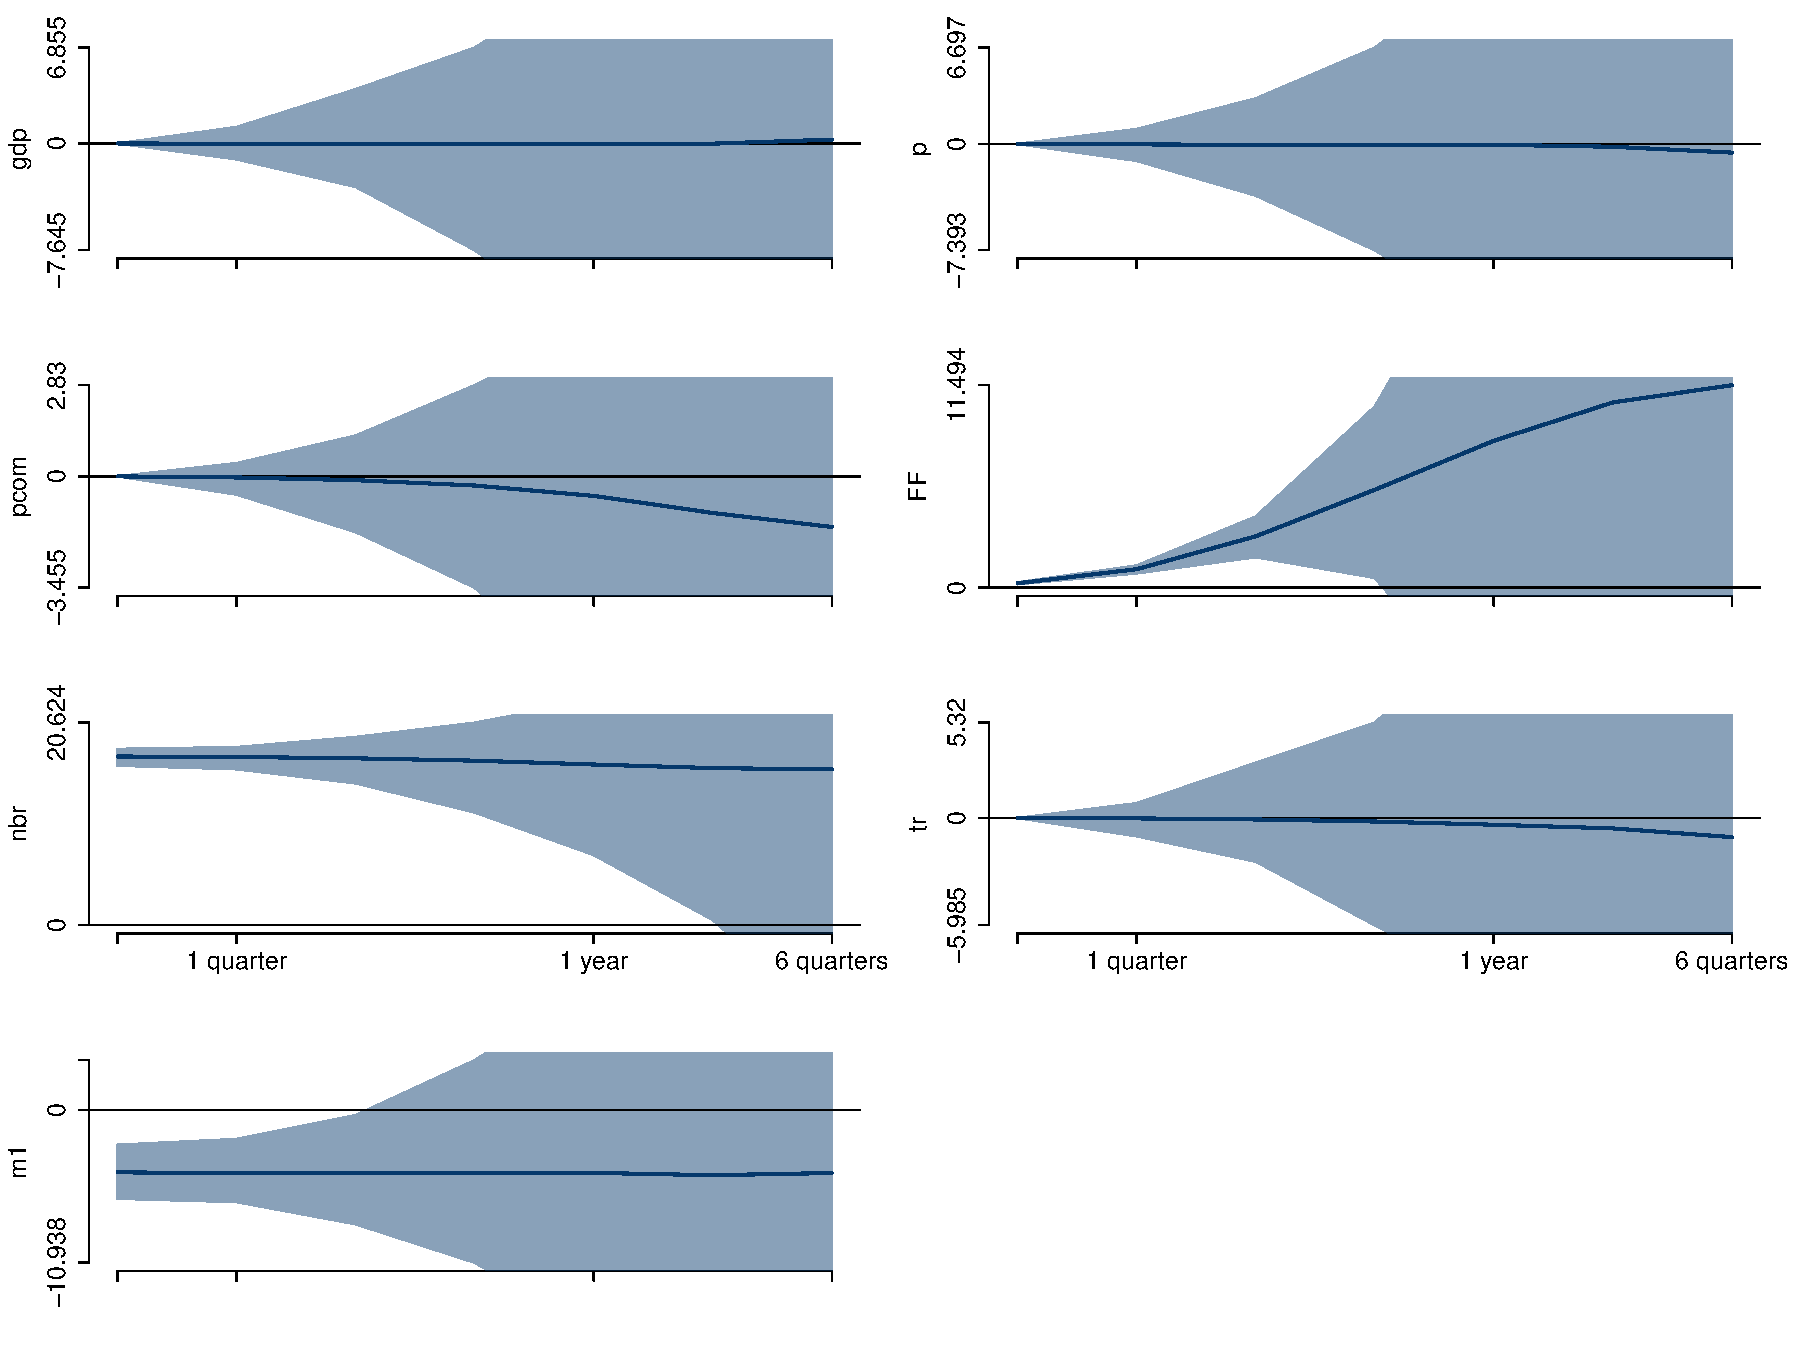
\includegraphics[scale=0.35]{NBRTR-irf-mps.pdf}

\end{frame}



{\setbeamercolor{background canvas}{bg=mcxs1}
\begin{frame}

\begin{center}
\vspace{1cm}\Large\textbf{\color{mcxs4}Modeling effects of monetary policy in the US}\\ \textbf{\color{mcxs2} Extended analysis}\\[3ex]
\textbf{\color{purple}Not Examinable}
\end{center}

\bigskip\footnotesize
\hspace{0.5cm}{\color{mcxs4} In reference to:}\\ 
\hspace{1cm}{\color{mcxs4} Christiano, Eichenbaum, \& Evans (1999, HM) }\\
\hspace{1cm}{\color{mcxs4} Ramey (2016, HM) }\\

\smallskip\hspace{0.5cm}{\color{mcxs4} as well as:}\\ 
\hspace{1cm}{\color{mcxs4} Normandin, Phaneuf (2004, JME) }\\
\hspace{1cm}{\color{mcxs4} Lanne, L\"utkepohl (2008, JEDC) }\\
\hspace{1cm}{\color{mcxs4} Wo\'zniak \& Droumaguet (2019) }\\

\end{frame}
}




\begin{frame}{Heteroskedastic Structural Vector Autoregressions}

\begin{align*}
{\color{purple}B_0} y_{t} &= b_0 + B_1 y_{t-1} + \dots + B_p y_{t-p} + u_t\\[1ex]
u_t|s_t &\sim \mathcal{N}\left( \mathbf{0}_N, {\color{purple}\text{diag}\left( \lambda_{s_t} \right)} \right)
\end{align*}

\begin{align*}
{\color{purple}B_{0.n}}&={\color{purple}b_n}V_n&& \text{-- restrictions for rows}\\
\sum_{s_t=1}^{M} \lambda_{n.s_t}&=1 && \text{-- standardization}\\[3ex]
s_t&=m\in\{1,\dots,M\}&& \text{-- Markov process}\\
\mathbf{P}&&& \text{-- transition matrix}\\
&(\kappa_1,\kappa_2,\kappa_4)&& \text{-- estimated hyper-parameters}\\
\end{align*}

\end{frame}




\begin{frame}
	\frametitle{Volatility of Structural Shocks}

\begin{center}
{\color{mcxs2}Marginal posterior state probabilities:} $\Pr[s_t|\mathbf{y}]$\\
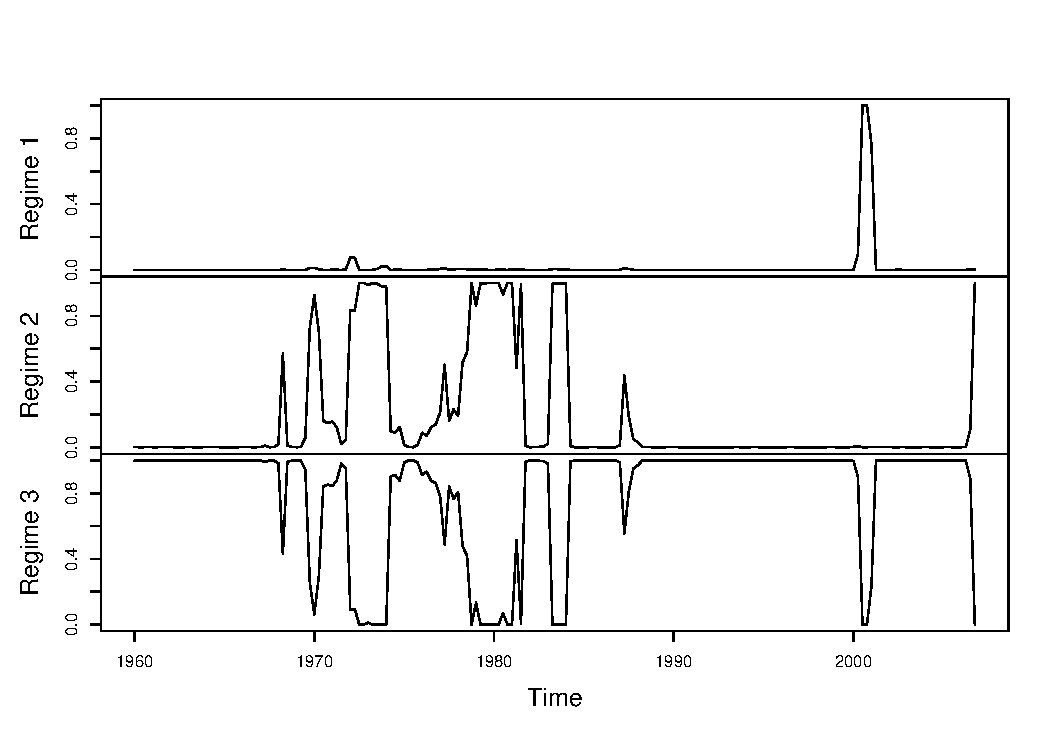
\includegraphics[scale=0.5]{./output-irfs/states-NBR-TR.pdf}
\end{center}    

\end{frame}





\begin{frame}
	\frametitle{Monetary Policy Models for  U.S. Data}


\begin{center}\small
\begin{tabular}{m{0.5cm} m{2.8cm} m{2.8cm} m{3.3cm}}
& FF  & NBR  & NBR-TR\\
$FF$& 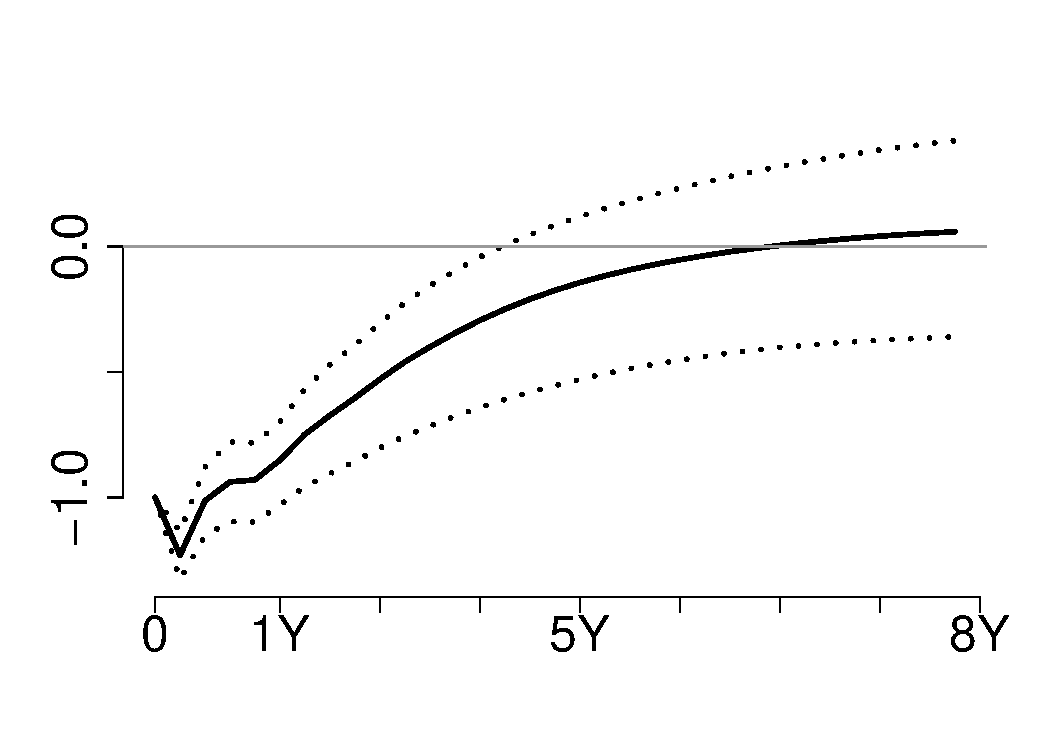
\includegraphics[scale=0.14]{./output-irfs/irf-ff-4.pdf} &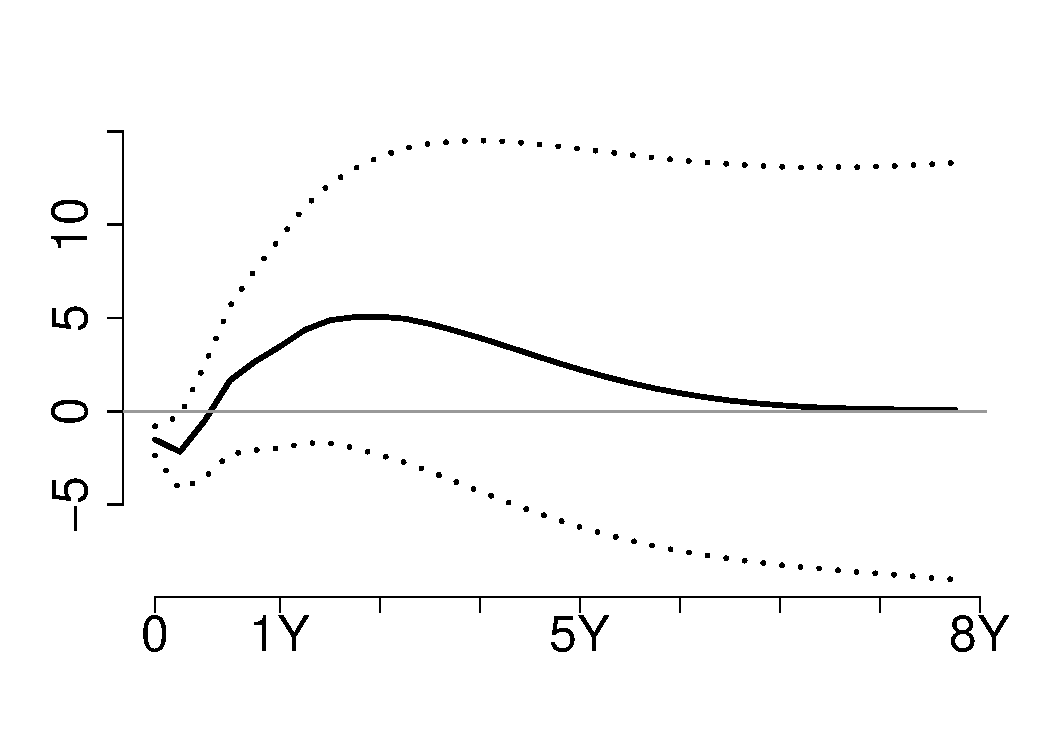
\includegraphics[scale=0.14]{./output-irfs/irf-nbr-4.pdf} & 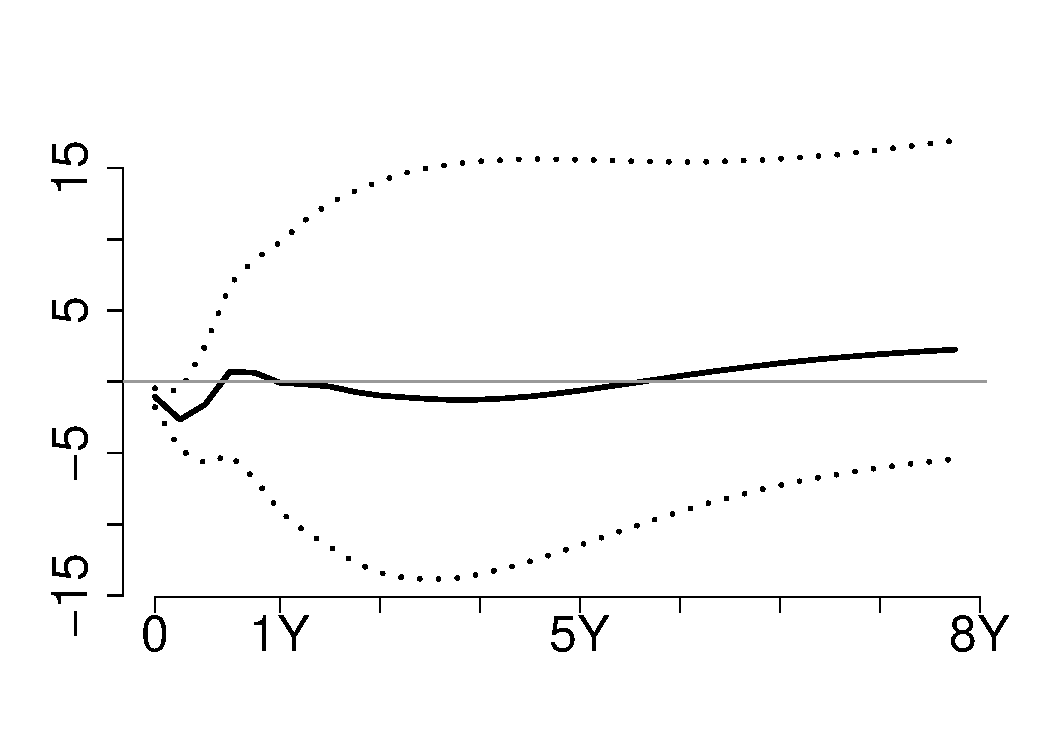
\includegraphics[scale=0.14]{./output-irfs/irf-nbrtr-4.pdf}\\
$nbr$& 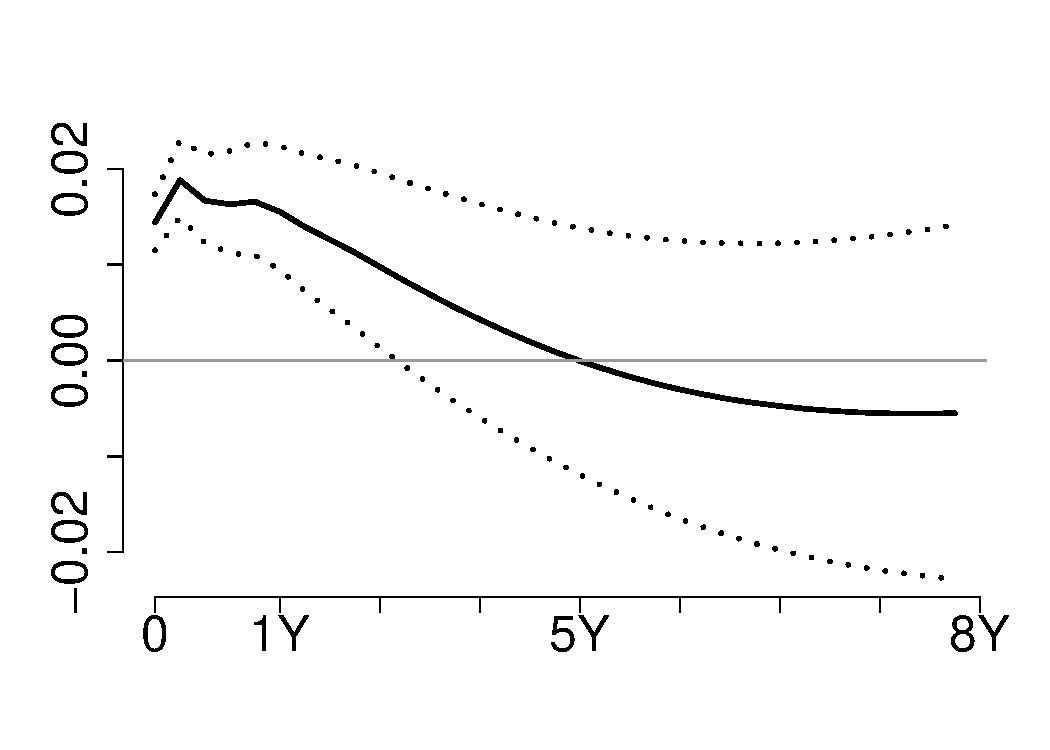
\includegraphics[scale=0.14]{./output-irfs/irf-ff-5.pdf} &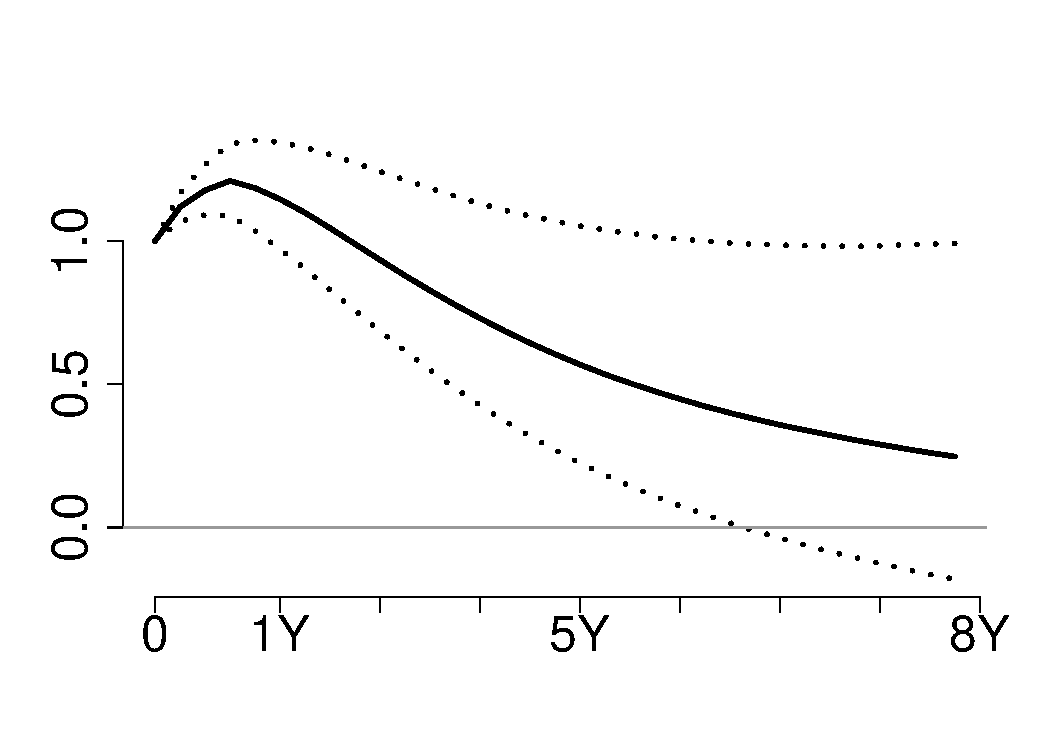
\includegraphics[scale=0.14]{./output-irfs/irf-nbr-5.pdf} & 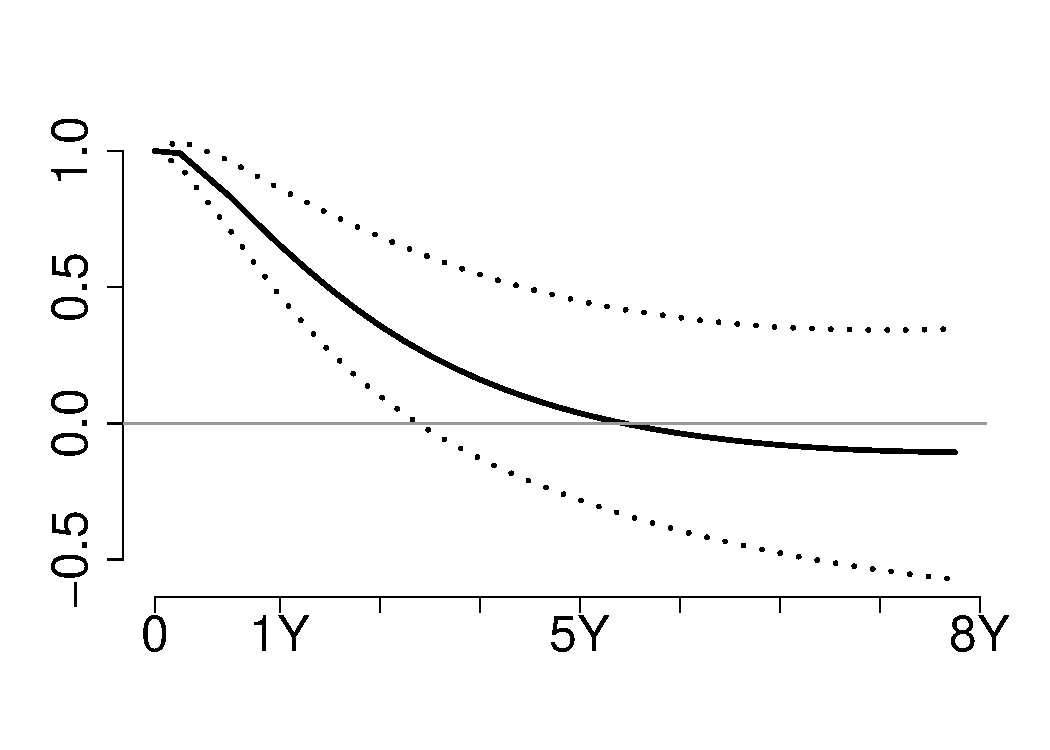
\includegraphics[scale=0.14]{./output-irfs/irf-nbrtr-5.pdf}\\
$tr$& 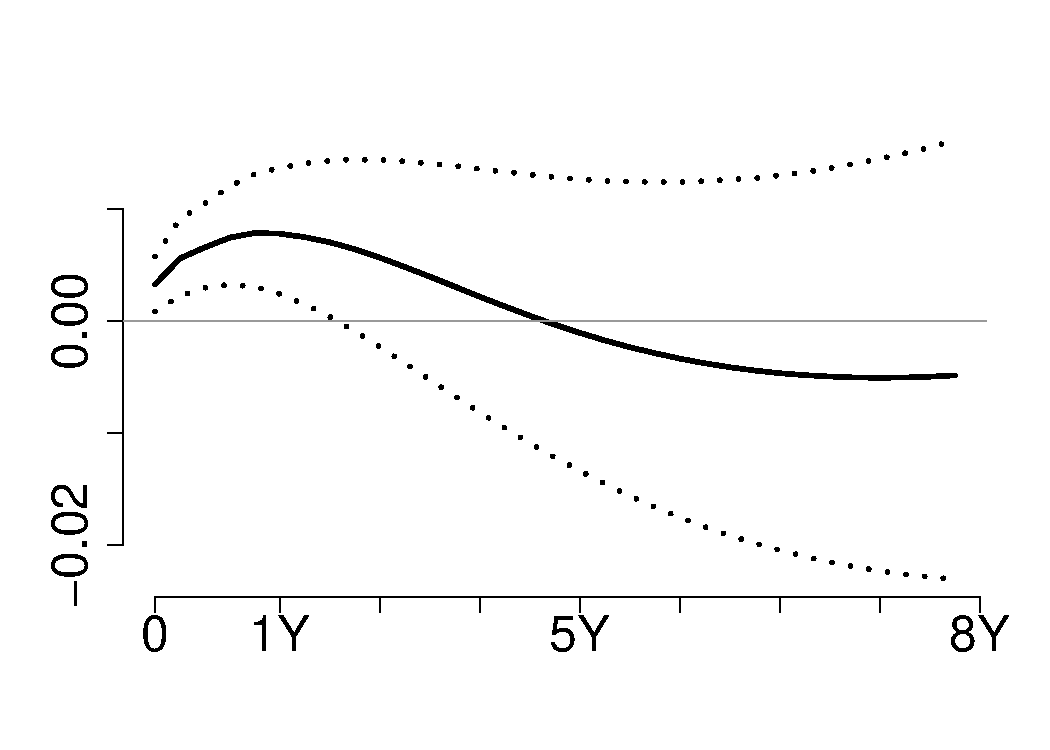
\includegraphics[scale=0.14]{./output-irfs/irf-ff-6.pdf} &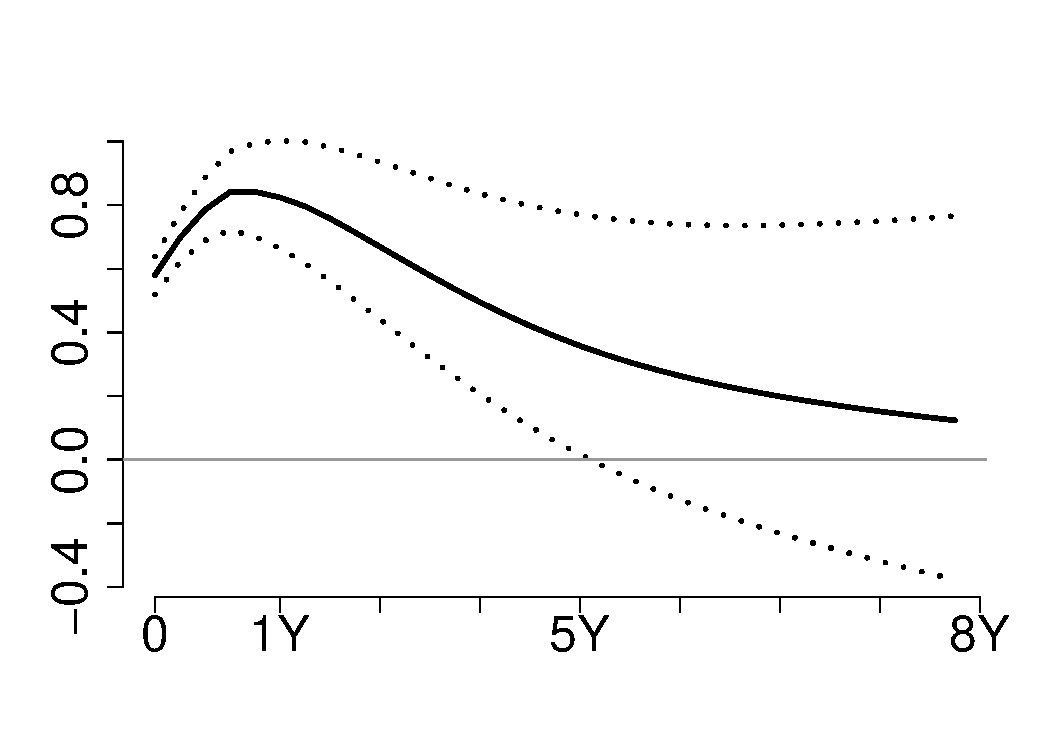
\includegraphics[scale=0.14]{./output-irfs/irf-nbr-6.pdf} & 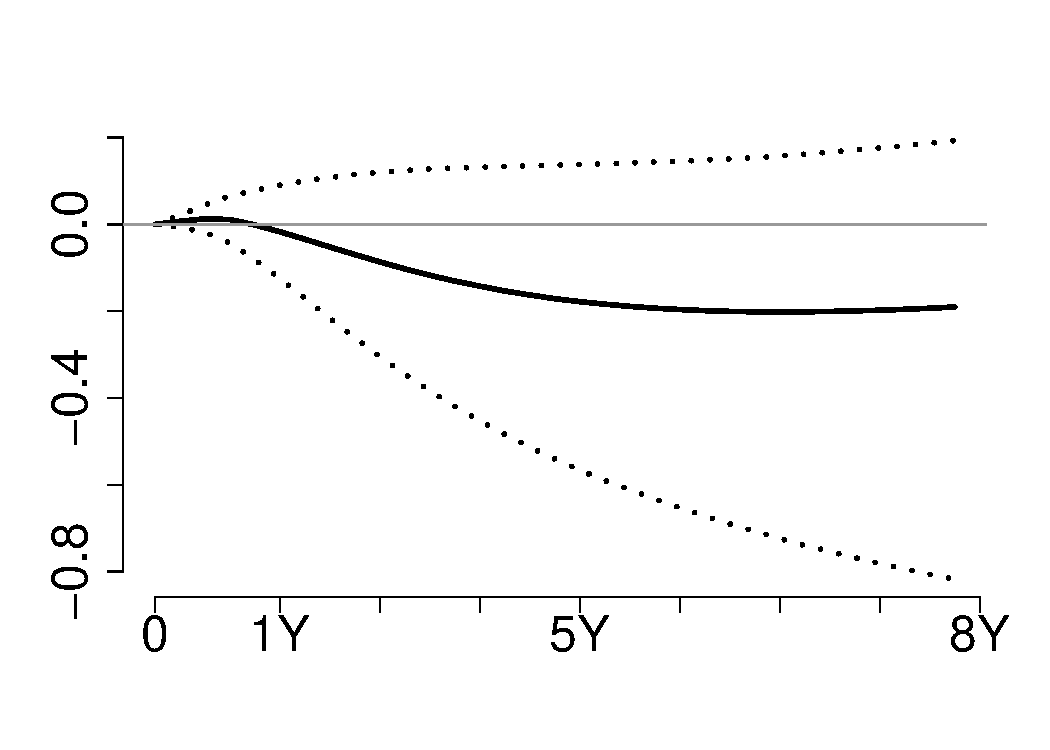
\includegraphics[scale=0.14]{./output-irfs/irf-nbrtr-6.pdf}\\
$m1$& 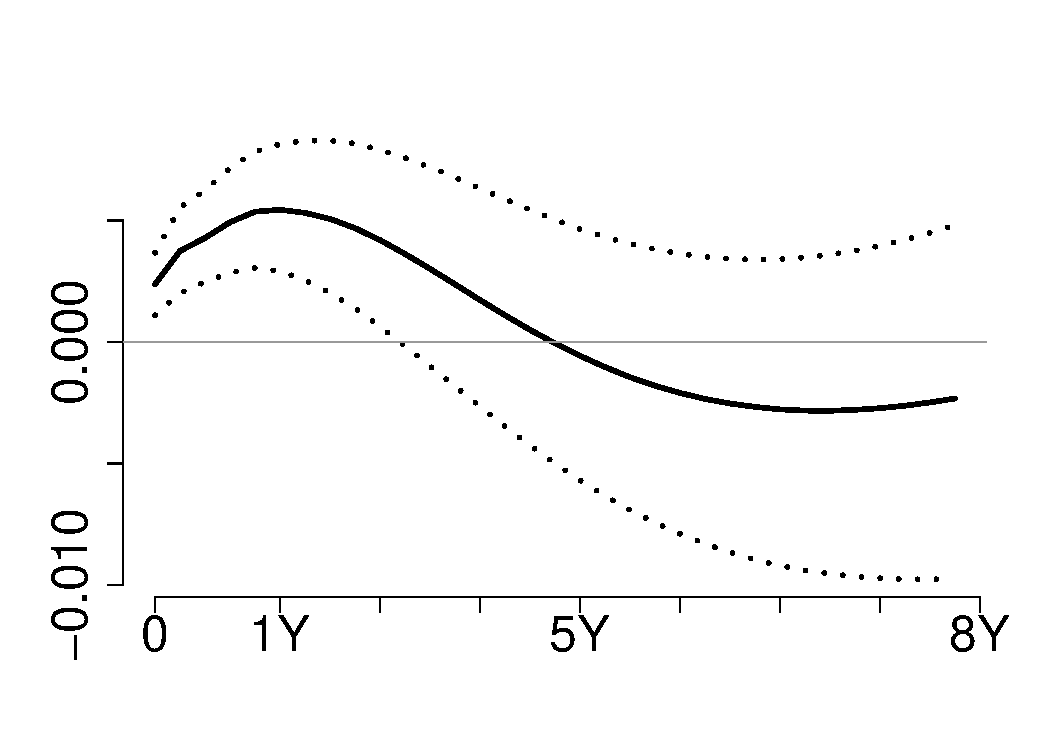
\includegraphics[scale=0.14]{./output-irfs/irf-ff-7.pdf} &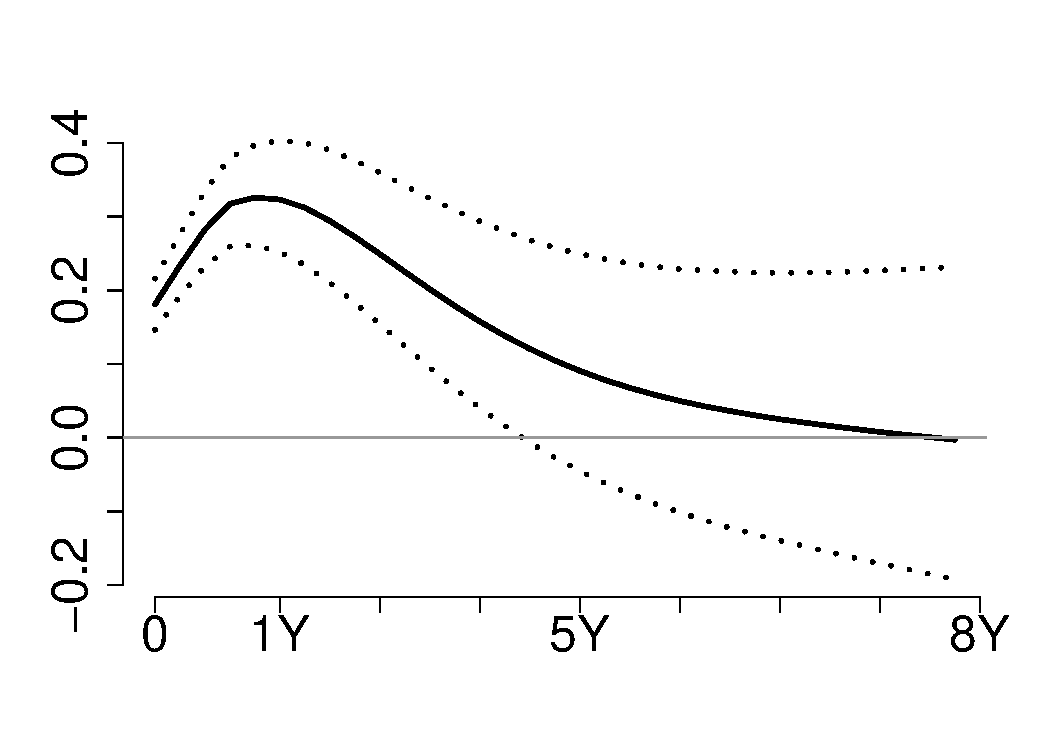
\includegraphics[scale=0.14]{./output-irfs/irf-nbr-7.pdf} & 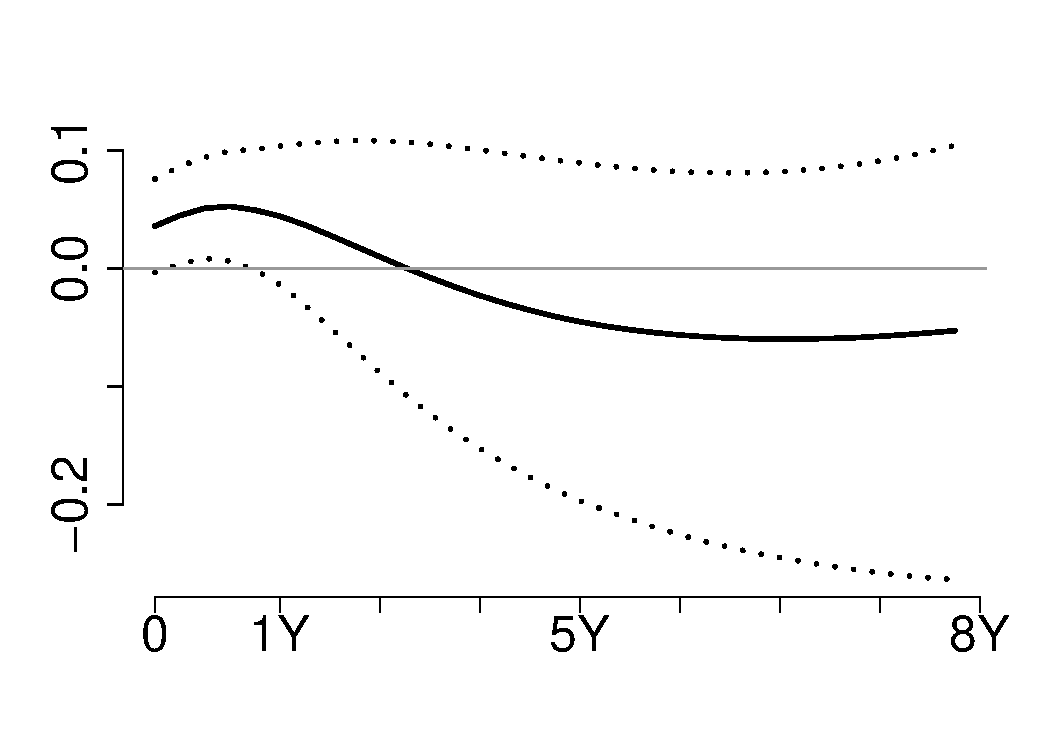
\includegraphics[scale=0.14]{./output-irfs/irf-nbrtr-7.pdf}
\end{tabular}
\end{center}

\end{frame}




\begin{frame}
	\frametitle{Monetary Policy Models for  U.S. Data}

\begin{center}\small
\begin{tabular}{m{0.5cm} m{2.8cm} m{2.8cm} m{3.3cm}}
& FF  & NBR  & NBR-TR\\
$gdp$ & 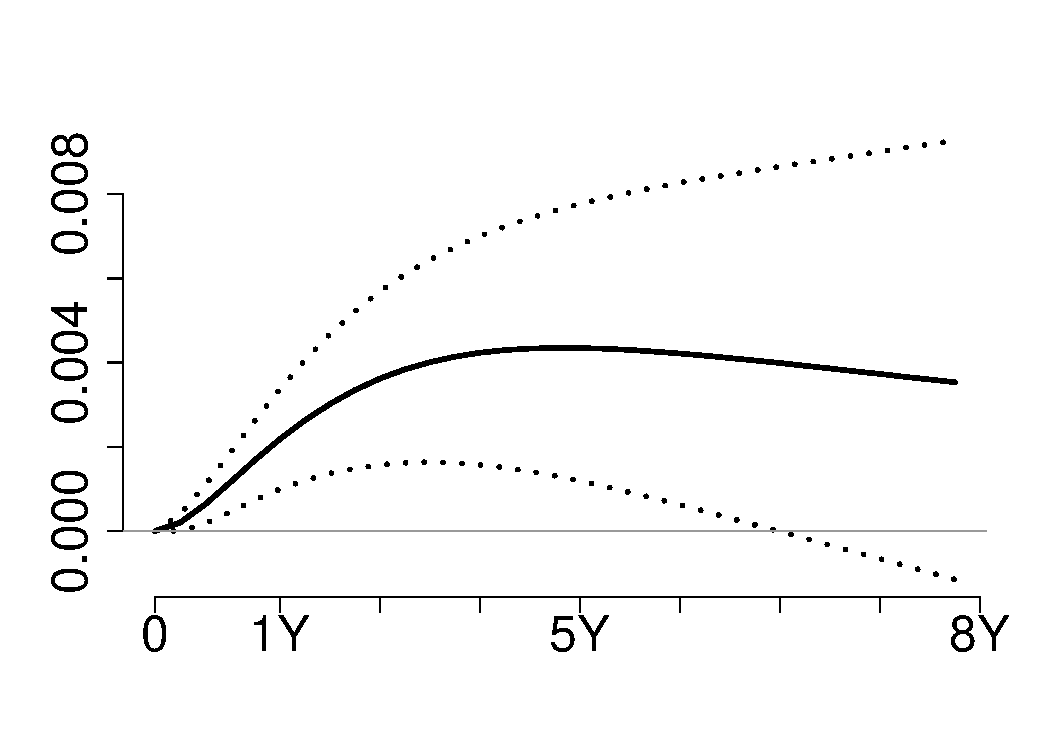
\includegraphics[scale=0.17]{./output-irfs/irf-ff-1.pdf} &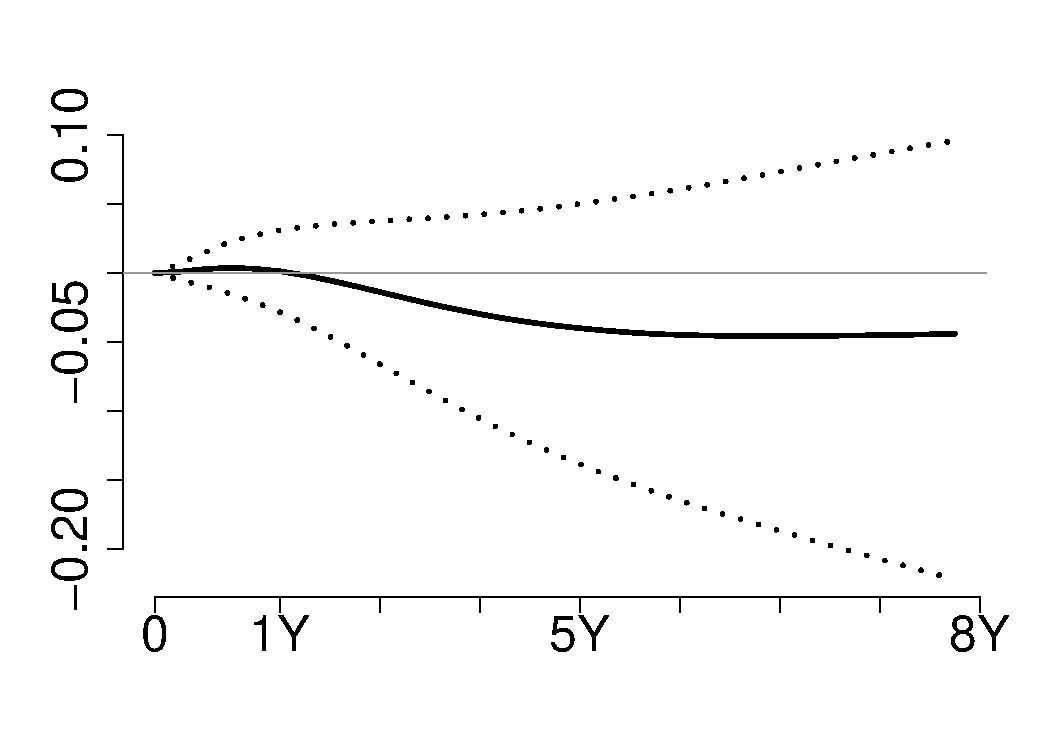
\includegraphics[scale=0.17]{./output-irfs/irf-nbr-1.pdf} & 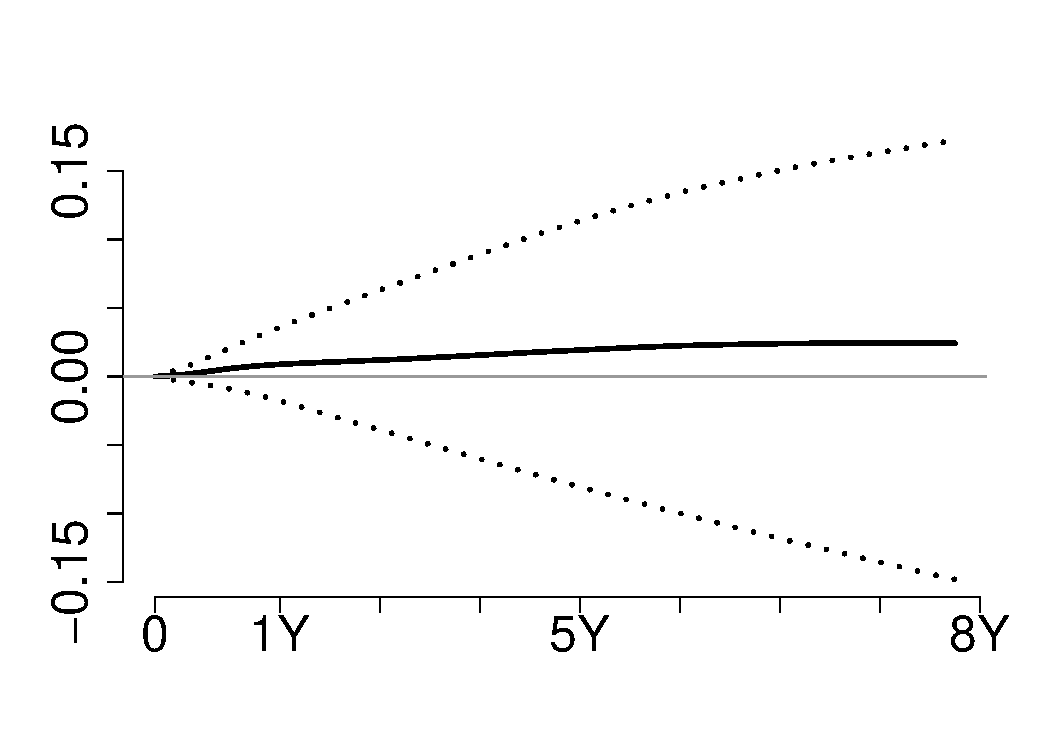
\includegraphics[scale=0.17]{./output-irfs/irf-nbrtr-1.pdf}\\
$p$& 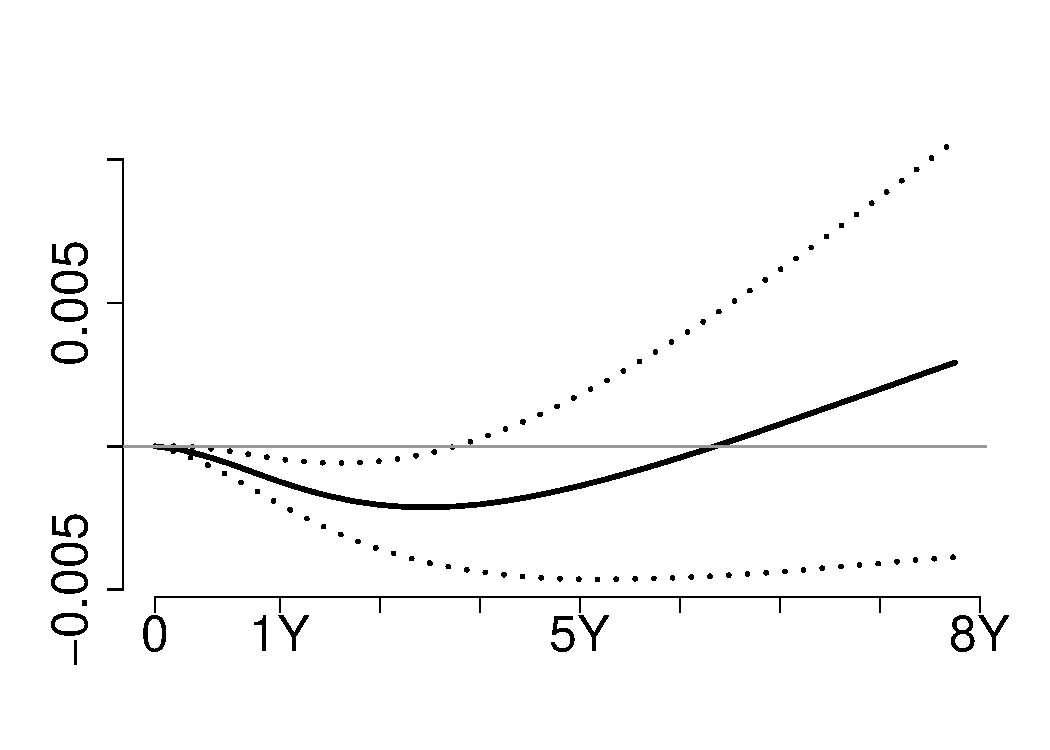
\includegraphics[scale=0.17]{./output-irfs/irf-ff-2.pdf} &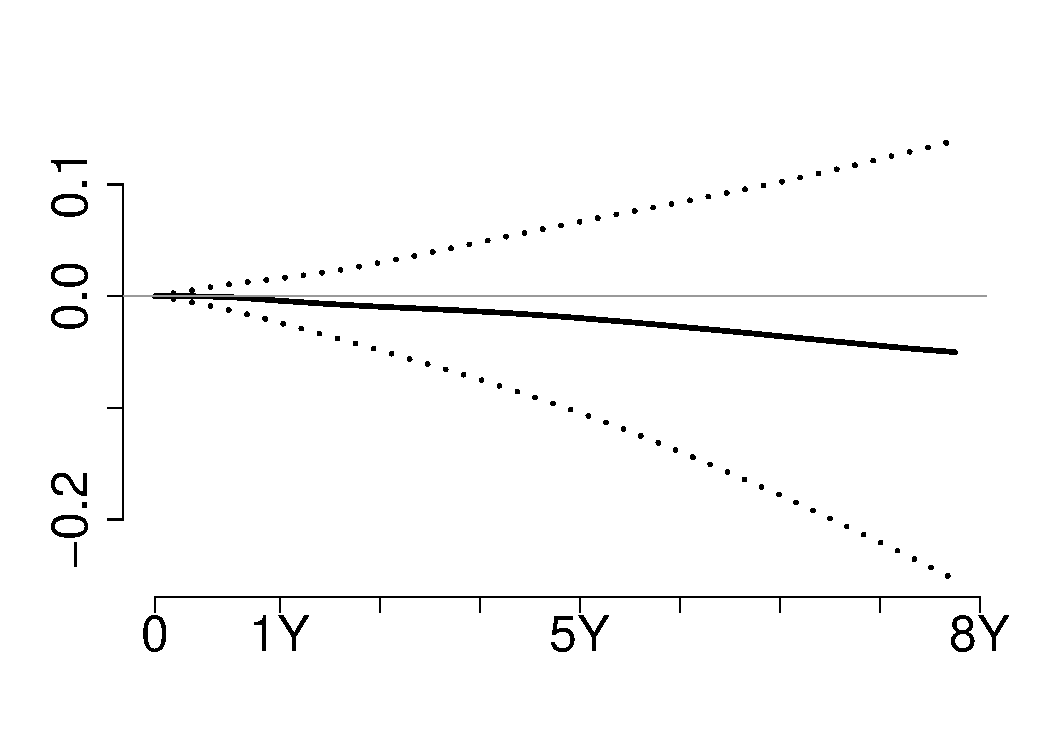
\includegraphics[scale=0.17]{./output-irfs/irf-nbr-2.pdf} & 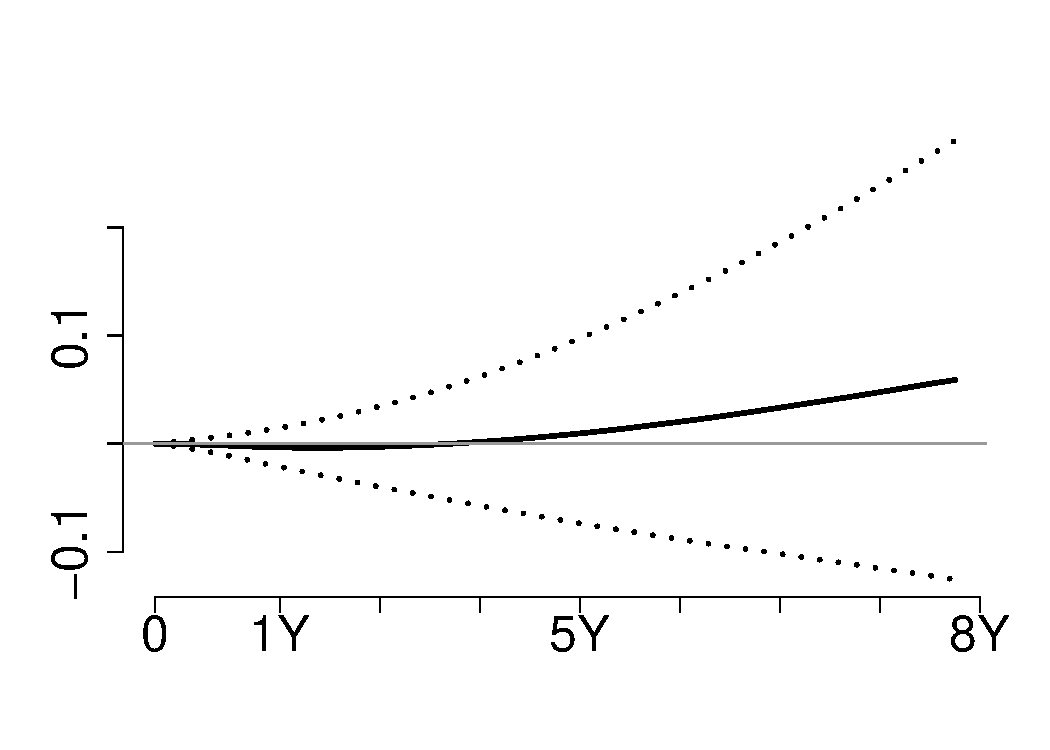
\includegraphics[scale=0.17]{./output-irfs/irf-nbrtr-2.pdf}\\
$pcom$& 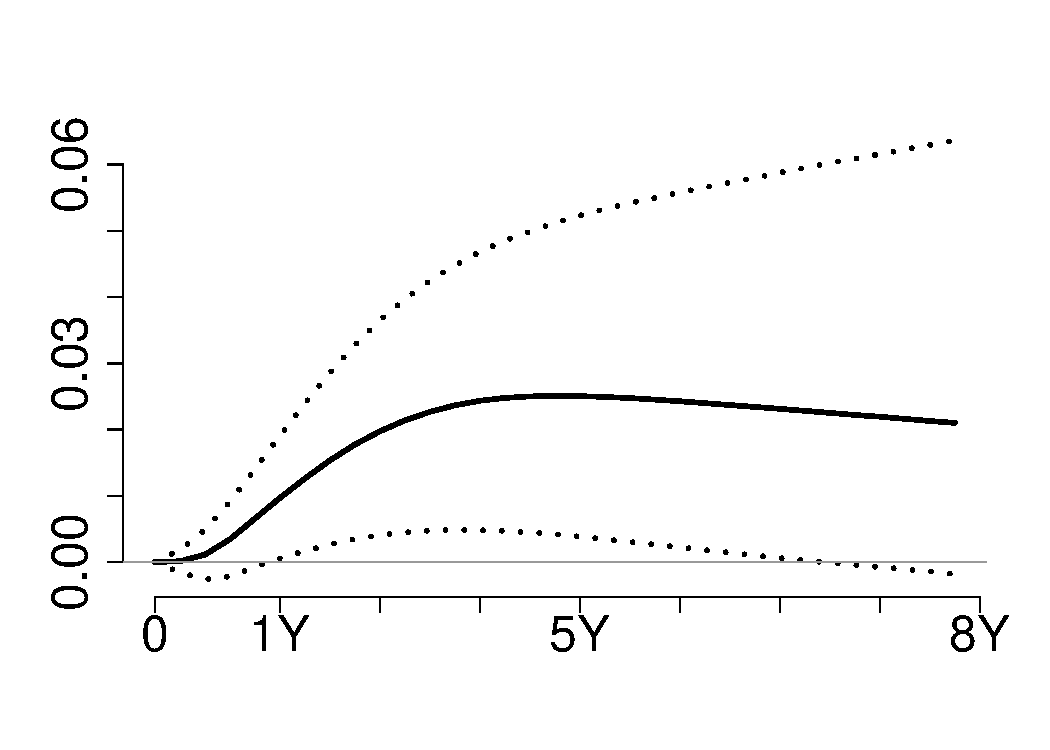
\includegraphics[scale=0.17]{./output-irfs/irf-ff-3.pdf} &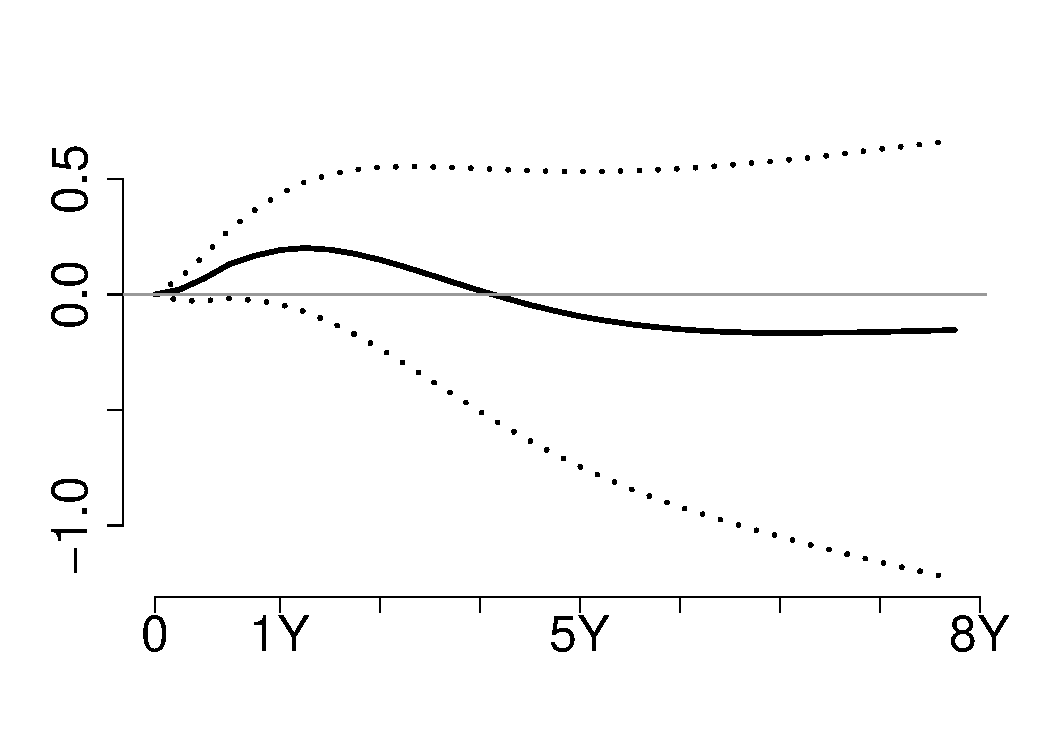
\includegraphics[scale=0.17]{./output-irfs/irf-nbr-3.pdf} & 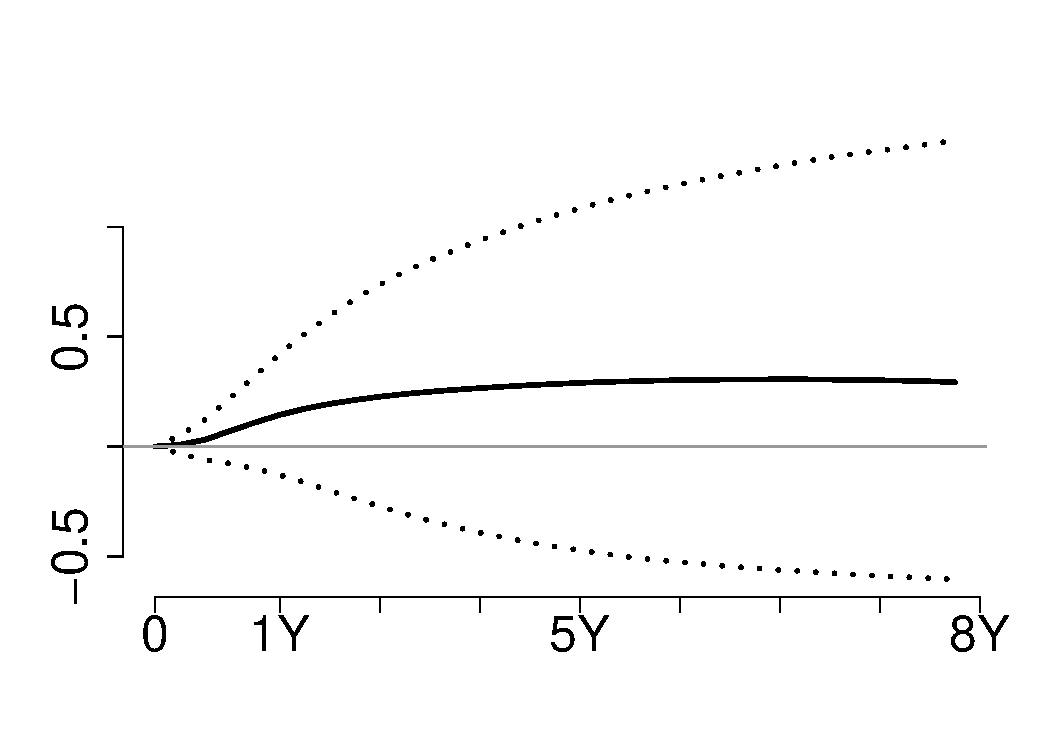
\includegraphics[scale=0.17]{./output-irfs/irf-nbrtr-3.pdf}
\end{tabular}
\end{center}

\end{frame}



\begin{frame}
	\frametitle{Identification Through Heteroskedasticity}

\textbf{Heteroskedasticity.}\\
{\color{mcxs2}Let there be} $2$ {\color{mcxs2}covariance matrices associated with data:}
$$ \Sigma_1,\quad\text{and}\quad\Sigma_2 $$

\bigskip\textbf{Contemporaneous effects matrix.}\\
{\color{mcxs2}All} $N^2$ {\color{mcxs2}elements of matrix} $B_0$ {\color{mcxs2}are identified:}
\begin{align*}
\Sigma_1 &= B_0^{-1}\text{diag}(\lambda_1)B_0^{-1'}\\
\Sigma_2 &= B_0^{-1}\text{diag}(\lambda_2)B_0^{-1'}
\end{align*}
\end{frame}





\begin{frame}
	\frametitle{Identification Through Heteroskedasticity}

\textbf{Heteroskedasticity.}\\
{\color{mcxs2}Let there be} $M$ {\color{mcxs2}covariance matrices associated with data:}
\begin{align*}
\Sigma_m &= B_0^{-1}\text{diag}(\lambda_m)B_0^{-1'}
\end{align*}


\bigskip\textbf{Contemporaneous effects matrix.}\\
{\color{mcxs2}All} $N^2$ {\color{mcxs2}elements of matrix} $B_0$ {\color{mcxs2}are identified.}

\bigskip{\color{mcxs2}Just-identifying restrictions in the homoskedastic case} \textbf{\color{purple}over identify the system in the heteroskedastic} {\color{mcxs2}one.}

\bigskip
\textbf{\color{purple}These restrictions can be tested!}

\end{frame}





\begin{frame}
	\frametitle{Monetary Policy Models for  U.S. Data}


\begin{table}[h]
\begin{center}\small
\begin{tabular}{ccccc}
\toprule
$M$ & Unrestricted & FF model & NBR model & NBR-TR model \\
\midrule
\multicolumn{5}{c}{\textit{Markov-switching heteroskedasticity}} \\
2& 2577.3& 2655.2& 2653.4& \textbf{2660.1} \\
3& 2660.6& 2710.0& 2708.2& \textbf{2731.4} \\
\bottomrule
\end{tabular}

\smallskip
Reported values: $\ln p(\mathbf{y}|\mathcal{M}_i)$ 
\end{center}
\end{table}





\end{frame}






\begin{frame}{References}
\scriptsize

\smallskip Bernanke \& Blinder (1992) {\color{mcxs2}The Federal Funds Rate and the Channels of Monetary Transmission American Economic Review}

\smallskip Christiano \& Eichenbaum (1992) {\color{mcxs2}Identification and the Liquidity Effect of a Monetary Policy Shock, Political Economy, Growth, and Business Cycles }

\smallskip Christiano, Eichenbaum \& Evans (1999) {\color{mcxs2}Monetary Policy Shocks: What Have We Learned and to What End? Handbook of Macroeconomics}

\smallskip Lanne, L\"utkepohl \& Maciejowska (2010) {\color{mcxs2}Structural vector autoregressions with Markov switching, Journal of Economic Dynamics and Control}

\smallskip Normandin \& Phaneuf (2004) {\color{mcxs2}Monetary policy shocks: Testing identification conditions under time-varying conditional volatility, Journal of Monetary Economics}

\smallskip Ramey (2016) {\color{mcxs2}Macroeconomic Shocks and Their Propagation, Handbook of Macroeconomics}

\smallskip Sims (1992) {\color{mcxs2}Interpreting the macroeonomic time series facts, The effects of monetary policy, European Economic Review}

\smallskip Strongin (1995) {\color{mcxs2}The identification of monetary policy disturbances explaining the liquidity puzzle, Journal of Monetary Economics }

\smallskip Uhlig (2005) {\color{mcxs2}What are the effects of monetary policy on output? Results from an agnostic identification procedure, Journal of Monetary Economics}

\smallskip Wo\'zniak \& Droumaguet (2019) {\color{mcxs2}Assessing Monetary Policy Models: Bayesian Inference for Heteroskedastic Structural VARs}

\end{frame}


\end{document} 